% !Mode:: "TeX:UTF-8"

\def\usewhat{pdflatex}                               % 定义编译方式 dvipdfmx 或者 pdflatex,默认为 dvipdfmx
                                                     % 方式编译,如果需要修改,只需改变花括号中的内容即可。
\documentclass[12pt,openany,oneside,ctexartutf8]{book}
                                                     % 本科生毕业论文通常采用单页排版
% !Mode:: "TeX:UTF-8"
%  Authors: 张井   Jing Zhang: prayever@gmail.com     天津大学2010级管理与经济学部信息管理与信息系统专业硕士生
%           余蓝涛 Lantao Yu: lantaoyu1991@gmail.com  天津大学2008级精密仪器与光电子工程学院测控技术与仪器专业本科生

%%%%%%%%%% Package %%%%%%%%%%%%
\usepackage{graphicx}                       % 支持插图处理
% \usepackage[a4paper,text={146.4true mm,239.2 true mm},top= 25.4true mm, bottom= 25.4true mm, left=31.7 true mm,head=6true mm,headsep=6.5true mm,foot=16.5true mm]{geometry}
\usepackage[a4paper,top=25.4mm, bottom=25.4mm, left=31.7mm, right=31.7mm, head=6true mm,headsep=6.5true mm,foot=17.5mm]{geometry}
                                            % 支持版面尺寸设置
\usepackage[squaren]{SIunits}               % 支持国际标准单位

\usepackage{titlesec}                       % 控制标题的宏包
\usepackage{titletoc}                       % 控制目录的宏包
\usepackage{fancyhdr}                       % fancyhdr宏包 支持页眉和页脚的相关定义
\usepackage[UTF8]{ctex}                     % 支持中文显示
\usepackage{CJKpunct}
\usepackage{color}                          % 支持彩色
\usepackage{amsmath}                        % AMSLaTeX宏包 用来排出更加漂亮的公式
\usepackage{amssymb}                        % 数学符号生成命令
\usepackage[below]{placeins}    %允许上一个section的浮动图形出现在下一个section的开始部分,还提供\FloatBarrier命令,使所有未处理的浮动图形立即被处理
\usepackage{multirow}                       % 使用Multirow宏包,使得表格可以合并多个row格
\usepackage{booktabs}                       % 表格,横的粗线;\specialrule{1pt}{0pt}{0pt}
\usepackage{longtable}                      % 支持跨页的表格。
\usepackage{tabularx}                       % 自动设置表格的列宽
\usepackage{subfigure}                      % 支持子图 %centerlast 设置最后一行是否居中
\usepackage[subfigure]{ccaption}            % 支持子图的中文标题
\usepackage[sort&compress,numbers]{natbib}  % 支持引用缩写的宏包
\usepackage{enumitem}                       % 使用enumitem宏包,改变列表项的格式
\usepackage{calc}                           % 长度可以用+ - * / 进行计算
\usepackage{txfonts}                        % 字体宏包
\usepackage{bm}                             % 处理数学公式中的黑斜体的宏包
\usepackage[amsmath,thmmarks,hyperref]{ntheorem}  % 定理类环境宏包,其中 amsmath 选项用来兼容 AMS LaTeX 的宏包
\usepackage{CJKnumb}                        % 提供将阿拉伯数字转换成中文数字的命令
\usepackage{indentfirst}                    % 首行缩进宏包
\usepackage{CJKutf8}                        % 用在UTF8编码环境下,它可以自动调用CJK,同时针对UTF8编码作了设置

% \usepackage{fancybox} 

%\usepackage{hypbmsec}                      % 用来控制书签中标题显示内容
\newcommand{\tabincell}[2]{\begin{tabular}{@{}#1@{}}#2\end{tabular}}
\usepackage{xcolor}
%支持代码环境
\usepackage{listings}
\lstset{numbers=left,
language=[ANSI]{C},
numberstyle=\tiny,
extendedchars=false,
showstringspaces=false,
breakatwhitespace=false,
breaklines=true,
captionpos=b,
keywordstyle=\color{blue!70},
commentstyle=\color{red!50!green!50!blue!50},
frame=shadowbox,
rulesepcolor=\color{red!20!green!20!blue!20}
}
%支持算法环境
\usepackage[boxed,ruled,lined]{algorithm2e}
\usepackage{algorithmic}

\usepackage{array}
\newcommand{\PreserveBackslash}[1]{\let\temp=\\#1\let\\=\temp}
\newcolumntype{C}[1]{>{\PreserveBackslash\centering}p{#1}}
\newcolumntype{R}[1]{>{\PreserveBackslash\raggedleft}p{#1}}
\newcolumntype{L}[1]{>{\PreserveBackslash\raggedright}p{#1}}

% 生成有书签的 pdf 及其生成方式。通常可以在 tjumain.tex 文件的第一行选择 pdflatex 或者是 dvipdfmx 编译手段。如果选择前者,则使用 pdflatex + pdflatex 编译; 如果选择后者,在编译的时候选择 latex + bibtex + latex + latex 编译。出现混淆的时候,系统会报错。
% 如果您的pdf制作中文书签有乱码使用如下命令,就可以解决了
\def\atemp{pdflatex}\ifx\atemp\usewhat
\usepackage{cmap}                           % pdflatex 编译时,可以生成可复制、粘贴的中文 PDF 文档, 缺点是在Windows上显示时效果不大好,字体发虚
\usepackage{hyperref}
\hypersetup{
    unicode,
    pdfborder={0 0 0},
}
\fi
% \usepackage[pdftex,unicode,
%             CJKbookmarks=true,
%             bookmarksnumbered=true,
%             bookmarksopen=true,
%             colorlinks=false,
%             pdfborder={0 0 0},
%             citecolor=blue,
%             linkcolor=red,
%             anchorcolor=green,
%             urlcolor=blue,
%             breaklinks=true
%             ]{hyperref}

                                % 定义本文所使用宏包
\graphicspath{{figures/}}                            % 定义所有的 .eps 文件在 figures 子目录下
\begin{document}                                     % 开始全文
\begin{CJK*}{UTF8}{song}                             % 开始中文字体使用
	% !Mode:: "TeX:UTF-8"
%  Authors: 张井   Jing Zhang: prayever@gmail.com     天津大学2010级管理与经济学部信息管理与信息系统专业硕士生
%           余蓝涛 Lantao Yu: lantaoyu1991@gmail.com  天津大学2008级精密仪器与光电子工程学院测控技术与仪器专业本科生

% 2018/5/23修正
%           李幼萌 Youmeng Li: liyoumeng@tju.edu.cn   天津大学软件学院软件工程系

%%%%%%%%%%%%%%%%% Fonts Definition and Basics %%%%%%%%%%%%%%%%%
\newcommand{\song}{\CJKfamily{song}}    % 宋体
\newcommand{\fs}{\CJKfamily{fs}}        % 仿宋体
\newcommand{\kai}{\CJKfamily{kai}}      % 楷体
\newcommand{\hei}{\CJKfamily{hei}}      % 黑体
\newcommand{\li}{\CJKfamily{li}}        % 隶书
\newcommand{\yihao}{\fontsize{26pt}{26pt}\selectfont}       % 一号, 单倍行距
\newcommand{\xiaoyi}{\fontsize{24pt}{24pt}\selectfont}      % 小一, 单倍行距
\newcommand{\erhao}{\fontsize{22pt}{1.25\baselineskip}\selectfont}       % 二号, 1.25倍行距
\newcommand{\xiaoer}{\fontsize{18pt}{18pt}\selectfont}      % 小二, 单倍行距
\newcommand{\sanhao}{\fontsize{16pt}{16pt}\selectfont}      % 三号, 单倍行距
\newcommand{\xiaosan}{\fontsize{15pt}{15pt}\selectfont}     % 小三, 单倍行距
\newcommand{\sihao}{\fontsize{14pt}{14pt}\selectfont}       % 四号, 单倍行距
\newcommand{\xiaosi}{\fontsize{12pt}{12pt}\selectfont}      % 小四, 单倍行距
\newcommand{\wuhao}{\fontsize{10.5pt}{10.5pt}\selectfont}   % 五号, 单倍行距
\newcommand{\xiaowu}{\fontsize{9pt}{9pt}\selectfont}        % 小五, 单倍行距

\CJKtilde  % 重新定义了波浪符~的意义
\newcommand\prechaptername{第}
\newcommand\postchaptername{章}

\punctstyle{hangmobanjiao}             % 调整中文字符的表示,行内占一个字符宽度,行尾占半个字符宽度

% 调整罗列环境的布局
\setitemize{leftmargin=3em,itemsep=0em,partopsep=0em,parsep=0em,topsep=-0em}
\setenumerate{leftmargin=3em,itemsep=0em,partopsep=0em,parsep=0em,topsep=0em}

% 避免宏包 hyperref 和 arydshln 不兼容带来的目录链接失效的问题。
\def\temp{\relax}
\let\temp\addcontentsline
\gdef\addcontentsline{\phantomsection\temp}

% 自定义项目列表标签及格式 \begin{publist} 列表项 \end{publist}
\newcounter{pubctr} %自定义新计数器
\newenvironment{publist}{%%%%%定义新环境
\begin{list}{[\arabic{pubctr}]} %%标签格式
    {
     \usecounter{pubctr}
     \setlength{\leftmargin}{2.5em}   % 左边界 \leftmargin =\itemindent + \labelwidth + \labelsep
     \setlength{\itemindent}{0em}     % 标号缩进量
     \setlength{\labelsep}{1em}       % 标号和列表项之间的距离,默认0.5em
     \setlength{\rightmargin}{0em}    % 右边界
     \setlength{\topsep}{0ex}         % 列表到上下文的垂直距离
     \setlength{\parsep}{0ex}         % 段落间距
     \setlength{\itemsep}{0ex}        % 标签间距
     \setlength{\listparindent}{0pt}  % 段落缩进量
    }}
{\end{list}}

\makeatletter
\renewcommand\normalsize{
  \@setfontsize\normalsize{12pt}{12pt} % 小四对应 12 pt
  \setlength\abovedisplayskip{4pt}
  \setlength\abovedisplayshortskip{4pt}
  \setlength\belowdisplayskip{\abovedisplayskip}
  \setlength\belowdisplayshortskip{\abovedisplayshortskip}
  \let\@listi\@listI}
\def\defaultfont{\renewcommand{\baselinestretch}{1.63}\normalsize\selectfont} % 设置行距

\renewcommand{\CJKglue}{\hskip -0.1 pt plus 0.08\baselineskip} % 控制字间距,使每行 34 个汉字
\makeatother

%%%%%%%%%%%%% Contents %%%%%%%%%%%%%%%%%
\renewcommand{\contentsname}{目\qquad 录}
\setcounter{tocdepth}{1} % 控制目录深度
\titlecontents{chapter}[2em]{\vspace{.5\baselineskip}\xiaosan\song}
             {\prechaptername\CJKnumber{\thecontentslabel}\postchaptername\qquad}{}
             {\hspace{.5em}\titlerule*[10pt]{$\cdot$}\sihao\contentspage}
\titlecontents{section}[4.2em]{\vspace{.25\baselineskip}\sihao\song}
             {\thecontentslabel\quad}{}
             {\hspace{.5em}\titlerule*[10pt]{$\cdot$}\sihao\contentspage}
% \titlecontents{subsection}[4em]{\vspace{.25\baselineskip}\xiaosi\song}
%              {\thecontentslabel\quad}{}
%              {\hspace{.5em}\titlerule*[10pt]{$\cdot$}\sihao\contentspage}

%%%%%%%%%% Chapter and Section %%%%%%%%%%%%%
\setcounter{secnumdepth}{4}
\setlength{\parindent}{2em}

\renewcommand{\chaptername}{\prechaptername\CJKnumber{\thechapter}\postchaptername}
\titleformat{\chapter}{\centering}{\xiaosan\song}{\chaptername}{} %{2em}
\titlespacing{\chapter}{0pt}{0.1\baselineskip}{0.8\baselineskip}

\titleformat{\section}{\sihao\hei}{\thesection}{1em}{}
\titlespacing{\section}{0pt}{0.15\baselineskip}{0.25\baselineskip}

\titleformat{\subsection}{\sihao\hei}{\thesubsection}{1em}{}
\titlespacing{\subsection}{0pt}{0.1\baselineskip}{0.3\baselineskip}

\titleformat{\subsubsection}{\sihao\hei}{\thesubsubsection}{1em}{}
\titlespacing{\subsubsection}{0pt}{0.05\baselineskip}{0.1\baselineskip}

%%%%%%%%%% Table, Figure and Equation %%%%%%%%%%%%%%%%%
\renewcommand{\tablename}{表}                                     % 插表题头
\renewcommand{\figurename}{图}                                    % 插图题头
\renewcommand{\thefigure}{\arabic{chapter}-\arabic{figure}}       % 使图编号为 7-1 的格式 %\protect{~}
\renewcommand{\thesubfigure}{\alph{subfigure})}                   % 使子图编号为 a) 的格式
\renewcommand{\thesubtable}{(\alph{subtable})}                    % 使子表编号为 (a) 的格式
\renewcommand{\thetable}{\arabic{chapter}-\arabic{table}}         % 使表编号为 7-1 的格式
\renewcommand{\theequation}{\arabic{chapter}-\arabic{equation}}   % 使公式编号为 7-1 的格式

%%%%%% 定制浮动图形和表格标题样式 %%%%%%
\makeatletter
\long\def\@makecaption#1#2{
   \vskip\abovecaptionskip
   \sbox\@tempboxa{\centering\wuhao\song{#1\qquad #2} }
   \ifdim \wd\@tempboxa >\hsize
     \centering\wuhao\song{#1\qquad #2} \par
   \else
     \global \@minipagefalse
     \hb@xt@\hsize{\hfil\box\@tempboxa\hfil}
   \fi
   \vskip\belowcaptionskip}
\makeatother
\captiondelim{~~~~} %用来控制longtable表头分隔符

%%%%%%%%%% Theorem Environment %%%%%%%%%%%%%%%%%
\theoremstyle{plain}
\theorembodyfont{\song\rmfamily}
\theoremheaderfont{\hei\rmfamily}
\newtheorem{theorem}{定理~}[chapter]
\newtheorem{lemma}{引理~}[chapter]
\newtheorem{axiom}{公理~}[chapter]
\newtheorem{proposition}{命题~}[chapter]
\newtheorem{prop}{性质~}[chapter]
\newtheorem{corollary}{推论~}[chapter]
\newtheorem{definition}{定义~}[chapter]
\newtheorem{conjecture}{猜想~}[chapter]
\newtheorem{example}{例~}[chapter]
\newtheorem{remark}{注~}[chapter]
%\newtheorem{algorithm}{算法~}[chapter]
\newenvironment{proof}{\noindent{\hei 证明:}}{\hfill $ \square $ \vskip 4mm}
\theoremsymbol{$\square$}

%%%%%%%%%% Page: number, header and footer  %%%%%%%%%%%%%%%%%

%\frontmatter 或 \pagenumbering{roman}
%\mainmatter 或 \pagenumbering{arabic}
\makeatletter
\renewcommand\frontmatter{\clearpage
  \@mainmatterfalse
  }
\makeatother

%%%%%%%%%%%% References %%%%%%%%%%%%%%%%%
\renewcommand{\bibname}{参考文献}
% 重定义参考文献样式,来自thu
\makeatletter
\renewenvironment{thebibliography}[1]{
    \titleformat{\chapter}{\raggedright\sihao\hei}{\chaptername}{2em}{}
   \chapter*{\bibname}
   \wuhao
   \list{\@biblabel{\@arabic\c@enumiv}}
        {\renewcommand{\makelabel}[1]{##1\hfill}
         \settowidth\labelwidth{0 cm}
         \setlength{\labelsep}{0pt}
         \setlength{\itemindent}{0pt}
         \setlength{\leftmargin}{\labelwidth+\labelsep}
         \addtolength{\itemsep}{-0.7em}
         \usecounter{enumiv}
         \let\p@enumiv\@empty
         \renewcommand\theenumiv{\@arabic\c@enumiv}}
    \sloppy\frenchspacing
    \clubpenalty4000
    \@clubpenalty \clubpenalty
    \widowpenalty4000
    \interlinepenalty4000
    \sfcode`\.\@m}
   {\def\@noitemerr
     {\@latex@warning{Empty `thebibliography' environment}}
    \endlist\frenchspacing}
\makeatother

\addtolength{\bibsep}{-0.5em}     % 缩小参考文献间的垂直间距
\setlength{\bibhang}{2em}         % 每个条目自第二行起缩进的距离

% 参考文献引用作为上标出现
%\newcommand{\citeup}[1]{\textsuperscript{\cite{#1}}}
\makeatletter
    \def\@cite#1#2{\textsuperscript{[{#1\if@tempswa , #2\fi}]}}
\makeatother
%% 引用格式
\bibpunct{[}{]}{,}{s}{}{,}

%%%%%%%%%%%% Cover %%%%%%%%%%%%%%%%%
% 封面、摘要、版权、致谢格式定义
\makeatletter
\def\ctitle#1{\def\@ctitle{#1}}\def\@ctitle{}
\def\cdegree#1{\def\@cdegree{#1}}\def\@cdegree{}
\def\caffil#1{\def\@caffil{#1}}\def\@caffil{}
\def\csubject#1{\def\@csubject{#1}}\def\@csubject{}
\def\cgrade#1{\def\@cgrade{#1}}\def\@cgrade{}
\def\cauthor#1{\def\@cauthor{#1}}\def\@cauthor{}
\def\cnumber#1{\def\@cnumber{#1}}\def\@cnumber{}
\def\cstuid#1{\def\@cstuid{#1}}\def\@cstuid{}
\def\cdate#1{\def\@cdate{#1}}\def\@cdate{}
\long\def\cabstract#1{\long\def\@cabstract{#1}}\long\def\@cabstract{}
\long\def\eabstract#1{\long\def\@eabstract{#1}}\long\def\@eabstract{}
\def\ckeywords#1{\def\@ckeywords{#1}}\def\@ckeywords{}
\def\ekeywords#1{\def\@ekeywords{#1}}\def\@ekeywords{}
\def\cheading#1{\def\@cheading{#1}}\def\@cheading{}
\def\ccovertitle#1{\def\@ccovertitle{#1}}\def\@ccovertitle{}

\pagestyle{fancy}
  \fancyhf{}
  \fancyhead[C]{\song\wuhao \@cheading}  % 页眉显示天津大学 20XX 届本科生毕业论文
  \fancyfoot[C]{\song\xiaowu ~\thepage~}
\newlength{\@title@width}

% 定义封面
\def\makecover{
%\cleardoublepage%
   \phantomsection
    \pdfbookmark[-1]{\@ctitle}{ctitle}

    \begin{titlepage}
      \vspace*{10pt}
      \begin{center}

      \begin{figure}[h]
      \centering
      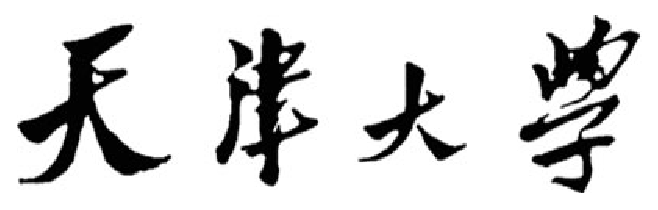
\includegraphics[width=0.4\textwidth]{figures/eps/tju}
      \end{figure}
      \vspace*{15pt}
      \hei\erhao{\textbf{\@ccovertitle}} \\
      \hei\erhao{\textbf{\@ctitle}}
      \vspace*{55pt}

      \begin{figure}[h]
      \centering
      
\includegraphics[width=0.3\textwidth]{figures/Tjulogo}
      \end{figure}

      \vspace*{60pt}
      \renewcommand\arraystretch{1.5}
      \setlength{\@title@width}{5cm}
      {
        \sanhao\song{
          \begin{tabular}{lc}
            \textbf{学\qquad 院}  &  \underline{\makebox[\@title@width][c]{\textbf{\@caffil}}} \\
            \textbf{专\qquad 业}  &  \underline{\makebox[\@title@width][c]{\textbf{\@csubject}}} \\
            \textbf{年\qquad 级}  &  \underline{\makebox[\@title@width][c]{\textbf{\@cgrade}}}\\
            \textbf{姓\qquad 名}  &  \underline{\makebox[\@title@width][c]{\textbf{\@cauthor}}}\\
            \textbf{学\qquad 号}  &  \underline{\makebox[\@title@width][c]{\textbf{\@cstuid}}}\\
          \end{tabular}
        }
    }
    \vspace*{40pt}

    \song\sanhao{\textbf{\@cdate}}
    \end{center}
    \end{titlepage}
}

                             % 完成对论文各个部分格式的设置
	% !Mode:: "TeX:UTF-8"


%%%%%%%%%%%%%%%%%%%%%%%%%%%%%%%%%%%%%%%%%%%%%%%%%%%%%%%%%%%%%%%
%%  可通过对 setup/format.tex中                               %%
%%  第243行 \setlength{\@title@width}{5cm}中 5cm 这个参数来   %%
%%  控制封面中下划线的长度。                                   %%
%%%%%%%%%%%%%%%%%%%%%%%%%%%%%%%%%%%%%%%%%%%%%%%%%%%%%%%%%%%%%%

\cheading{天津大学软件学院~\the\year~年《专业课程设计2》结课报告}      % 正文页眉
\ccovertitle{《专业课程设计2》结课报告}                       % 封面标题

%%%%%%%%%%%%%%%%%%%%%%%%%%%%%%%%%%%%%%%%%%%%%%%%%%%%%%%%%%%%%
%%%%%%%%%% 以下为论文的基本信息,需要由作者进行修改 %%%%%%%%%%%%
%%%%%%%%%%%%%%%%%%%%%%%%%%%%%%%%%%%%%%%%%%%%%%%%%%%%%%%%%%%%%
\ctitle{基于ESP8266的局域网控制检测系统}    % 封面用论文标题,自己可手动断行
\caffil{智能与计算学部}       % 学院名称
\csubject{软件工程}     % 专业名称
\cgrade{2017级}           % 年级
\cauthor{姓名}          % 学生姓名
\cstuid{1234567890}     % 学号

\cdate{\the\year~年~\the\month~月~\the\day~日}  % 论文完成日期,不需要修改,自动生成

	\frontmatter                                     % 以下是论文导言部分,包括论文的封面,中英文摘要和中文目录
	\fancypagestyle{plain}{							 % 正文前均无页眉
		\fancyhf{}
		\renewcommand{\headrulewidth}{0 pt}
		\fancyfoot[C]{\song\xiaowu~\thepage~}
	}

	\makecover 			% 封面

	% !Mode:: "TeX:UTF-8"

% 目录
\defaultfont
\clearpage{
    \pagestyle{empty}
    \cleardoublepage
    \setcounter{page}{1}                                 % 单独从 1 开始编页码
    \pagenumbering{arabic}
    \titleformat{\chapter}{\centering\sanhao\hei}{\chaptername}{2em}{} % 设置目录两字的格式
    \pdfbookmark[0]{目~~录}{mulu}
    \tableofcontents                                     % 中文目录
    \thispagestyle{plain}
} % 目录

	\mainmatter\defaultfont\sloppy\raggedbottom
	\makeatletter
	\fancypagestyle{plain}{                              % 设置正文眉页脚风格
		\fancyhf{}
		\fancyhead[C]{\song\wuhao \@cheading}            % 页眉格式
		\fancyfoot[C]{\song\xiaowu ~\thepage~}           % 页脚格式
		\renewcommand{\headrulewidth}{0.5pt}
		\renewcommand{\footrulewidth}{0pt}
	}
	\makeatother
	\setcounter{page}{1}                                 % 单独从 1 开始编页码
	\titleformat{\chapter}{\centering\xiaosan\hei}{\chaptername}{2em}{} % 恢复chapter标题格式要求

	%%%%%% 这里是正文,每个文件对应正文中的一章 %%%%%%
	% !Mode:: "TeX:UTF-8"

\chapter{需求概述}
\section{项目背景}

当今,随着物质生活水平的提高和网络的普及,人们对于生活条件的要求也日益提高,因此基于物联网的智能家居应运而生。

而ESP8266是一款超低功耗的UART-WiFi透传模块,拥有业内极富竞争力的封装尺寸和超低能耗技术,专为移动设备和物联网应用设计,可将用户的物理设备连接到Wi-Fi 无线网络上,进行互联网或局域网通信,实现联网功能。ESP8266可广泛应用于智能电网、智能交通、智能家具、手持设备、工业控制等领域。

在此背景之下,我们小组选择利用ESP8266制作一个网络控制检测系统,简单模拟智能家居的工作原理,进而向智能家居方向发展。

\section{项目需求}

项目的实际需求是旨在利用型号为ESP8266的单片机的WiFi模组,结合各种传感器,实现对家庭中的部分电器设备的远程操控和对家庭环境状况的远程监控。

最终产品的具体功能有:远程控制LED灯的开关,方便用户对于家电的控制;实时监测室内温度湿度数值以及变化曲线,便于用户了解室内环境情况;检测室内烟雾情况以及是否出现明火并及时发出警报,提供了非常快捷灵敏的警报系统,为用户的安全提供了有力的保障;此外,使用红外检测,实现人来灯亮、人走灯灭的全自动化功能,让用户体验到更加人性化的功能。

本产品的具体实现方式为Android手机APP和Web网页两种方式,手机APP为用户提供了便捷、便携、便利的使用体验,而Web网页为用户提供了双重保障,从而进一步提升用户体验。

\section{条件限制}

\begin{enumerate}
    \item 由于实际电路中电压太高,存在一定的安全风险,而且电路连接不方便,所以用LED灯代替电灯。
    \item 由于一台ESP8266只有一个ADC口,不能同时接多个传感器,所以用两个单片机同时工作。
    \item 由于远程网络通信更加复杂,所以暂时实现局域网内数据通信。
\end{enumerate}
	% !Mode:: "TeX:UTF-8"

\chapter{团队人员分工}
\section{团队成员(按学号排序)}
\begin{itemize}
    \item {3017218159}: 李琛
    \item {3017218164}: 石琦
    \item {3017218179}: 赵崇阳
    \item {3017218180}: 赵鸿博
\end{itemize}
\section{人员分工(按学号排序)}
\begin{enumerate}
    \item {李琛}: 
    
        负责Web页面开发,搭建Web Server,实现Web页面与单片机数据互通。
    \item {石琦}: 
    
        负责电路连接,用单片机获取传感器数据;搭建TCP Server,实现单片机与Android端数据互通。
    \item {赵崇阳}: 
    
        负责Android端UI界面的初步设计,以及课程设计报告的初步撰写。
    \item {赵鸿博}: 
    
        进行Android端UI界面的设计,负责APP功能的实现,以及与单片机进行的TCP通讯。
\end{enumerate}
	% !Mode:: "TeX:UTF-8"

\chapter{项目设计}
\section{实现形式}

在最初的设计中,我们预计使用两种方式来实现我们对室内设备的控制,以及显示对室内环境状况的监测。一个是移动端的Android APP,另一个是Web端的网页。预期设计的界面如下:

\begin{figure}[htbp]
\centering
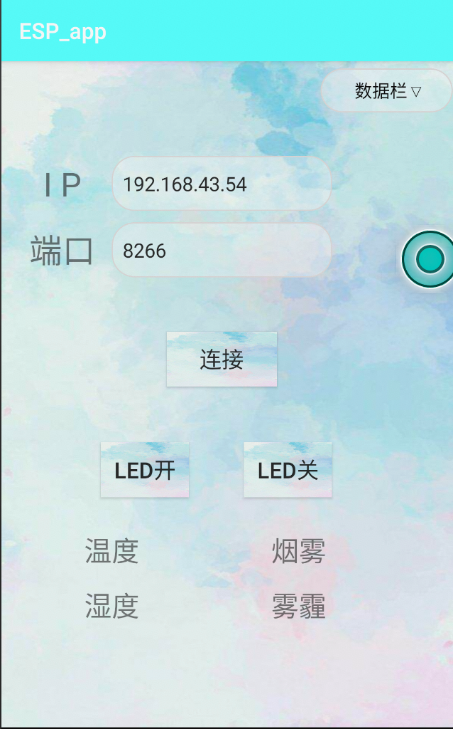
\includegraphics[width=0.3\textwidth]{figures/app_UI}
\caption{App界面}\label{fig:1}
\end{figure}

\begin{figure}[htbp]
\centering
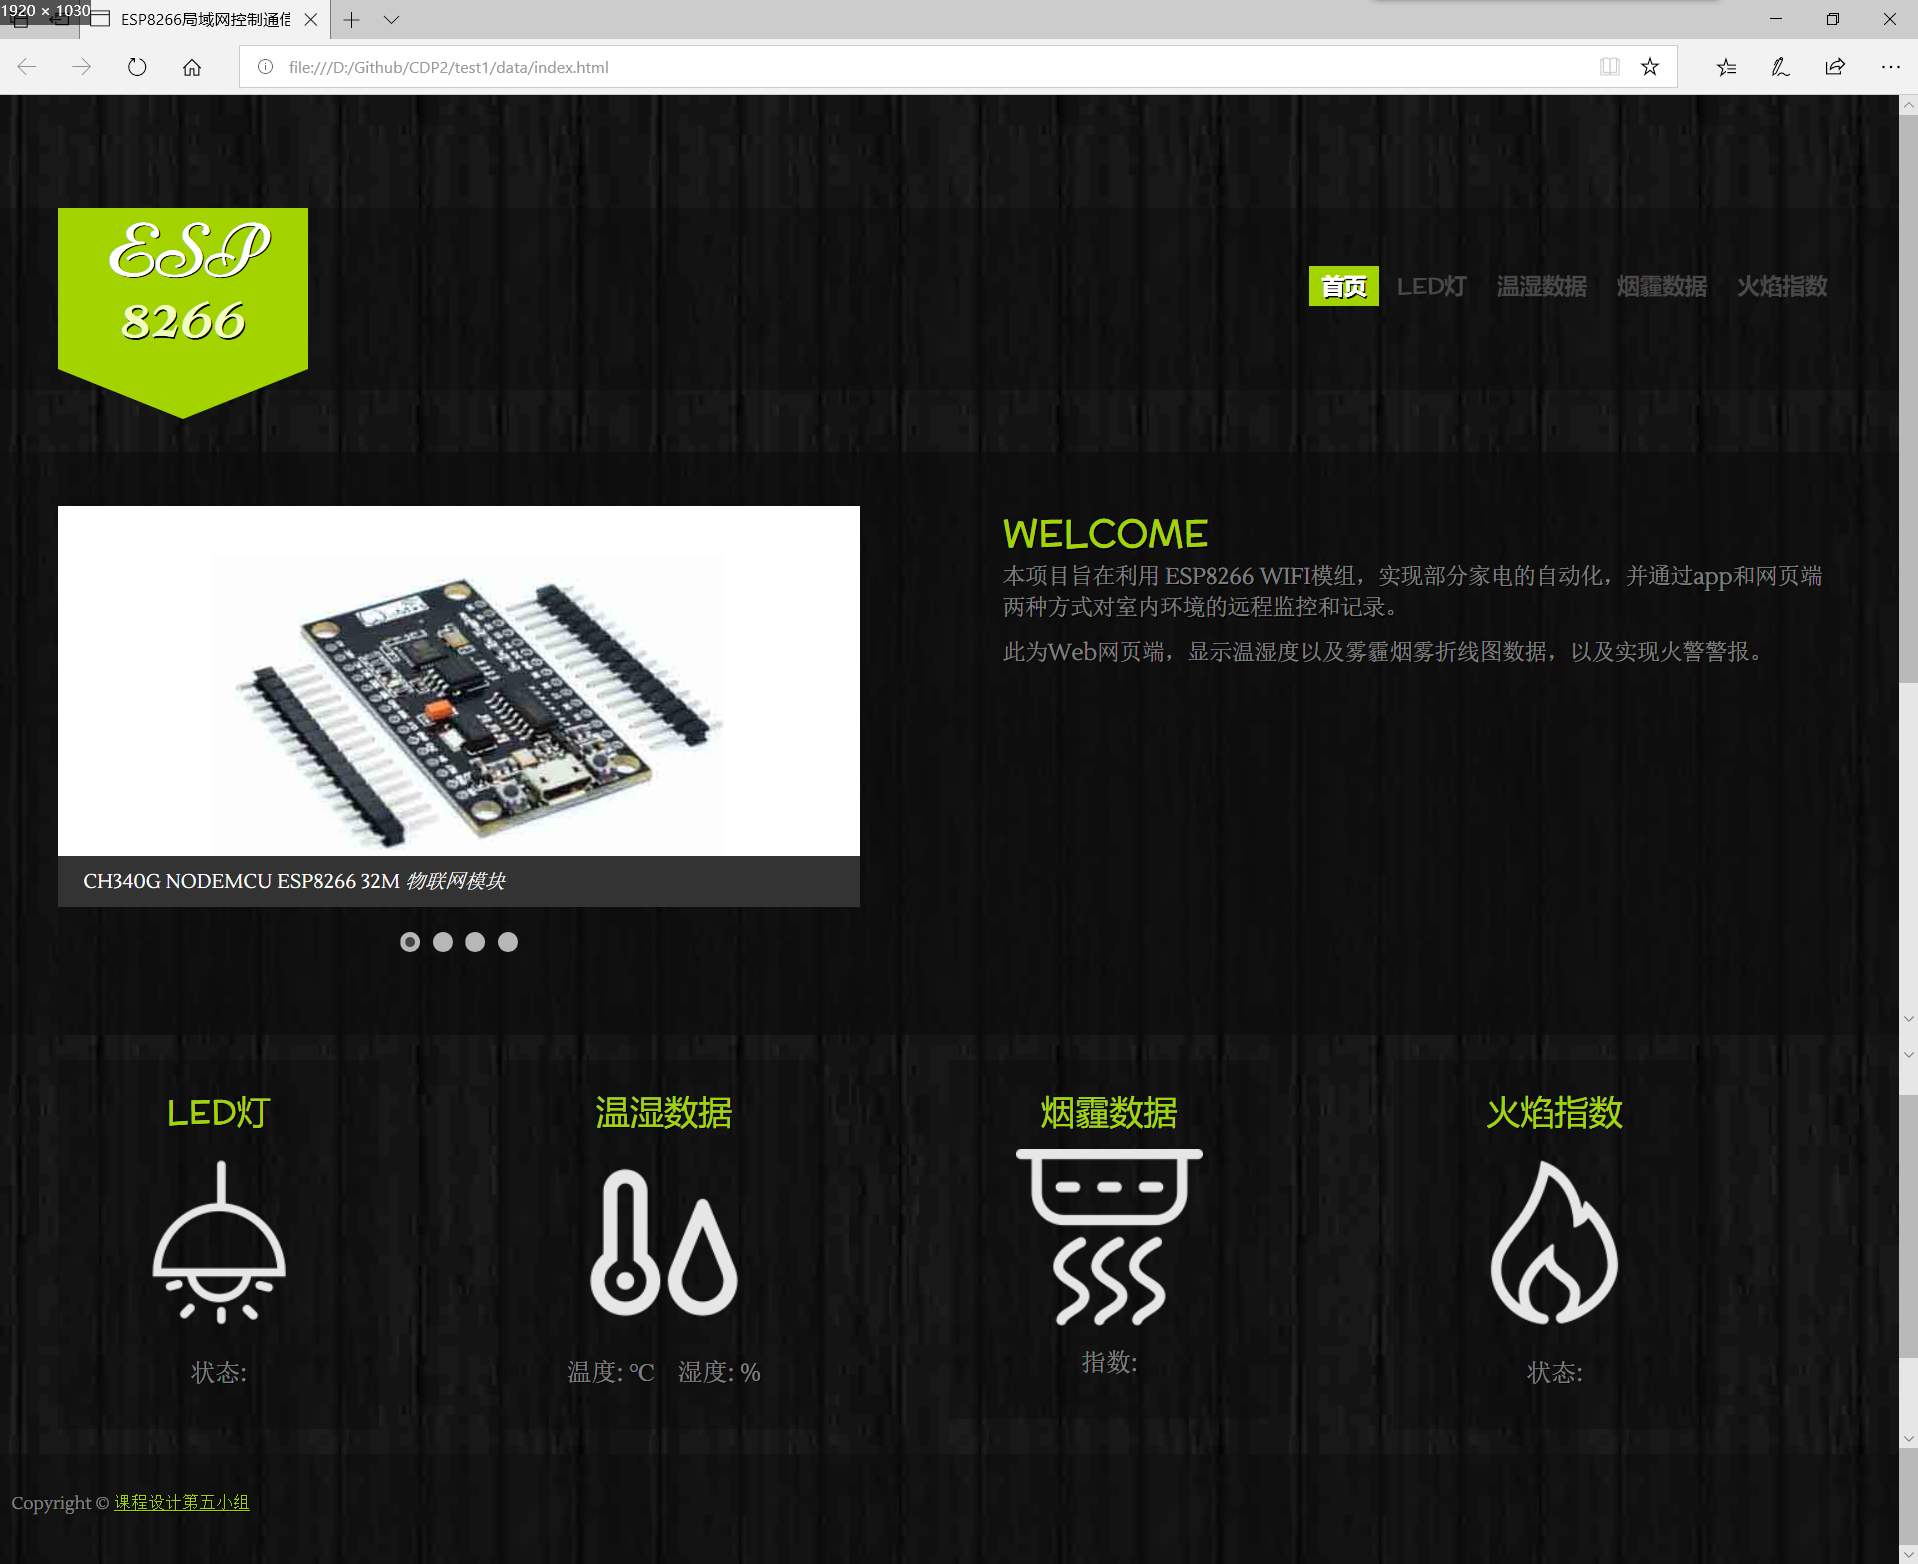
\includegraphics[width=0.7\textwidth]{figures/web_UI}
\caption{Web界面}\label{fig:2}
\end{figure}

\section{使用器材}

\begin{enumerate}
    \item {单片机ESP8266物联网模块}: 
    
    在项目设计的实际相关内容中,核心的部件是单片机ESP8266物联网模块,通过在其中烧录代码,使它能够对移动端app或者是web端发送的指令进行响应,并将传感器读取的数据传回app或是web上。实物如下:
    \begin{figure}[htbp]
    \centering
    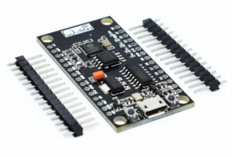
\includegraphics[width=0.3\textwidth]{figures/esp8266}
    \caption{CH340G NODEMCU ESP8266 32M 物联网模块}\label{fig:3}
    \end{figure}

    \item {温湿度传感器}:
    
    对于室内环境状况检测的功能设计中,我们设计了对温度和湿度数据的采集和记录功能。主要采用的是传感器DHT11 温湿度传感器(实物如下图)。通过DHT11 温湿度传感器获取了温度和湿度数据后,再通过ESP8266传回移动端app与web端,使其能够直观地显示出来。除了可以获取当前的温度和湿度数据。我们同样再app和web网页上设计了数据折线图
。按照一定的时间周期,记录温度和湿度数据,绘制成历史数据折线图。可以更明了清晰地观察到室内环境的变化情况。
    \begin{figure}[htbp]
    \centering
    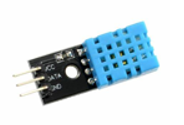
\includegraphics[width=0.3\textwidth]{figures/dht11}
    \caption{DHT11 温湿度传感器}\label{fig:4}
    \end{figure}

    \item {人体红外感应模块}:
    
    在对室内的部分设备进行控制的内容设计上,我们主要设计的是对led灯的开关控制功能,通过连接到ESP8266 WiFi局域网上,可以通过移动端手机app或者是PC端的web网页对led灯的开关进行远程控制。除了可以使用远程开关对led进行控制,我们还设计了“人过灯亮、人走灯灭”的自动开关灯,主要是通过传感器HC-SR501 人体红外感应模块(实物如下)采集红外感应数据,并让程序对获取的数据进行分析,实现自动的开关灯。
    \begin{figure}[htbp]
    \centering
    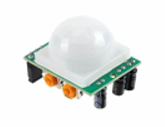
\includegraphics[width=0.3\textwidth]{figures/hongwai}
    \caption{HC-SR501 人体红外感应模块}\label{fig:5}
    \end{figure}

    \item {灰尘传感器}:
    
    室内环境状况检测的功能中,我们还设计了室内烟霾指数的测量与记录功能。主要使用的是传感器GP2Y1010AU0F 灰尘传感器(实物如下图),这个传感器可以检测室内空气中的灰尘与烟霾浓度,并将采集到的实时数据通过ESP8266传回app与web网页进行显示。与温度和湿度数据的采集和记录方式类似,除了获取当前的烟霾指数数据,我们同样设计了用于显示数据变化的折线图,在移动端app和web端上分别按照一定时间间隔绘制历史数据折线图,可以直观地反映烟霾指数变化情况。
    \begin{figure}[htbp]
    \centering
    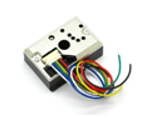
\includegraphics[width=0.3\textwidth]{figures/huichen}
    \caption{GP2Y1010AU0F 灰尘传感器}\label{fig:6}
    \end{figure}

    \item {火焰传感器+蜂鸣器}:
    
    最后一项功能是火灾报警装置。我们设计了结合蜂鸣器和火焰传感器(实物如下图)的火灾报警装置,火焰传感器获取室内烟雾和温度等数据,并判断是否室内起火,如果确定起火则将信号传递给蜂鸣器,触发蜂鸣器发出警报。

    \begin{figure}
        \centering
        \begin{minipage}{0.4\textwidth}
            \centering
            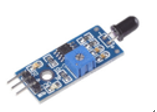
\includegraphics[width=0.5\textwidth]{figures/huoyan}
            \caption{火焰传感器}\label{fig:7}    
        \end{minipage}
        \begin{minipage}{0.4\textwidth}
            \centering
            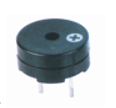
\includegraphics[width=0.4\textwidth]{figures/fengming}
            \caption{蜂鸣器}\label{fig:8}    
        \end{minipage}
    \end{figure}
\end{enumerate}
	% !Mode:: "TeX:UTF-8"

\chapter{项目过程}

\section{电路连接及数据获取}

\section{WiFi模块服务器搭建}

在单片机与Web端数据通信时,采用HTTP协议,使用ESP8266的STA模式,即单片机作为客户端,连接到局域网内进行数据互通。

关于搭建Web Server,我们采用了ESP8266提供的ESP8266WebServer功能,实现步骤如下:

\begin{enumerate}
    \item 引入相应的库\#include  \textless ESP8266WebServer.h\textgreater;
    \item 建立全局的Web服务器并监听某端口ESP8266WebServer server(port);(port一般可写80) 
    \item 在setup()中绑定http请求的回调函数server.on(url, function);
    \item 在setup()中绑定http请求不可用时的回调函数server.onNotFound(function);
    \item 在setup()中开启WebServer功能server.begin();
    \item 在loop()中监听客户请求并处理server.handleClient();
\end{enumerate}

部分关键代码如下:

\begin{figure}[htbp]
    \centering
    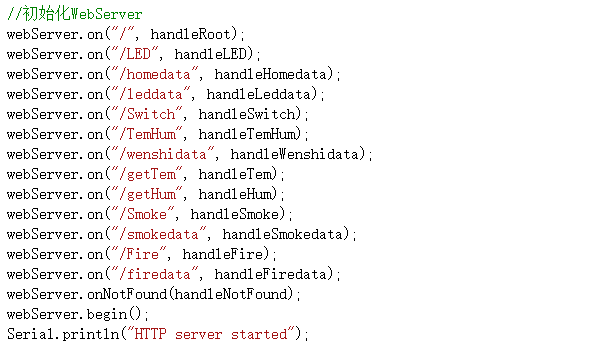
\includegraphics[width=0.8\textwidth]{figures/code/1}
    \caption{初始化WebServer}
\end{figure}

\begin{figure}[htbp]
    \centering
    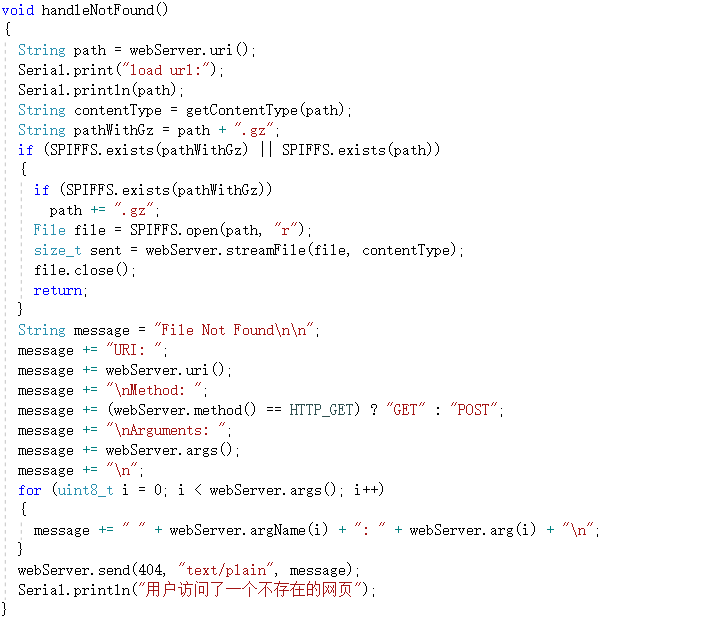
\includegraphics[width=0.8\textwidth]{figures/code/2}
    \caption{handleNotFound()方法}
\end{figure}

\begin{figure}[htbp]
    \centering
    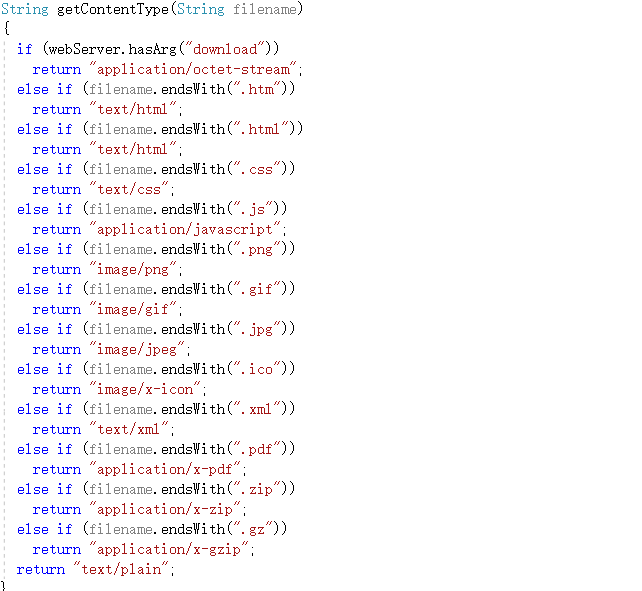
\includegraphics[width=0.8\textwidth]{figures/code/3}
    \caption{getContentType()方法}
\end{figure}

\section{APP界面设计及数据通信}

\begin{enumerate}

\item {APP UI界面设计}:

通过Android Studio的LinearLayout基础框架设计主界面,使用了2个TextView,2个EditText以及一个Button制作TCP连接登陆框架;使用了2个Button制作ESP8266上连接小灯的开关控制;使用了4个TextView制作温湿度以及烟霾数据的时时数据显示窗口;使用了Spinner(下拉菜单)制作查看温湿度历史数据折线图,烟霾历史数据折线图等界面的自由跳转功能。

两个历史数据折线图界面均使用LinearLayout基础框架设计,包含一个TextView显示主题,一个HelloChart的LineChartView绘制折线图,其中HelloChart为Android Studio制作折线图,柱状图等图表的开源库。

\item {APP界面通过Spinner控件自由跳转实现}:

Spinner控件通过Adapter以及Click监听实现Activity之间的切换,通过辨别点击不同的item来跳转相应界面,并使用Intent和Bundle来进行数据的传递,以保证历史数据的存储方便绘制历史折线图。由于Spinner控件最初若连续点击相同item不会进行响应只会对有别于之前选中的选项进行事件响应,所以使用AdapterView中的事件绑定的方式更改相同事件可重复进行的变量,实现点击相同item仍进行跳转。

\begin{figure}[htbp]
    \centering
    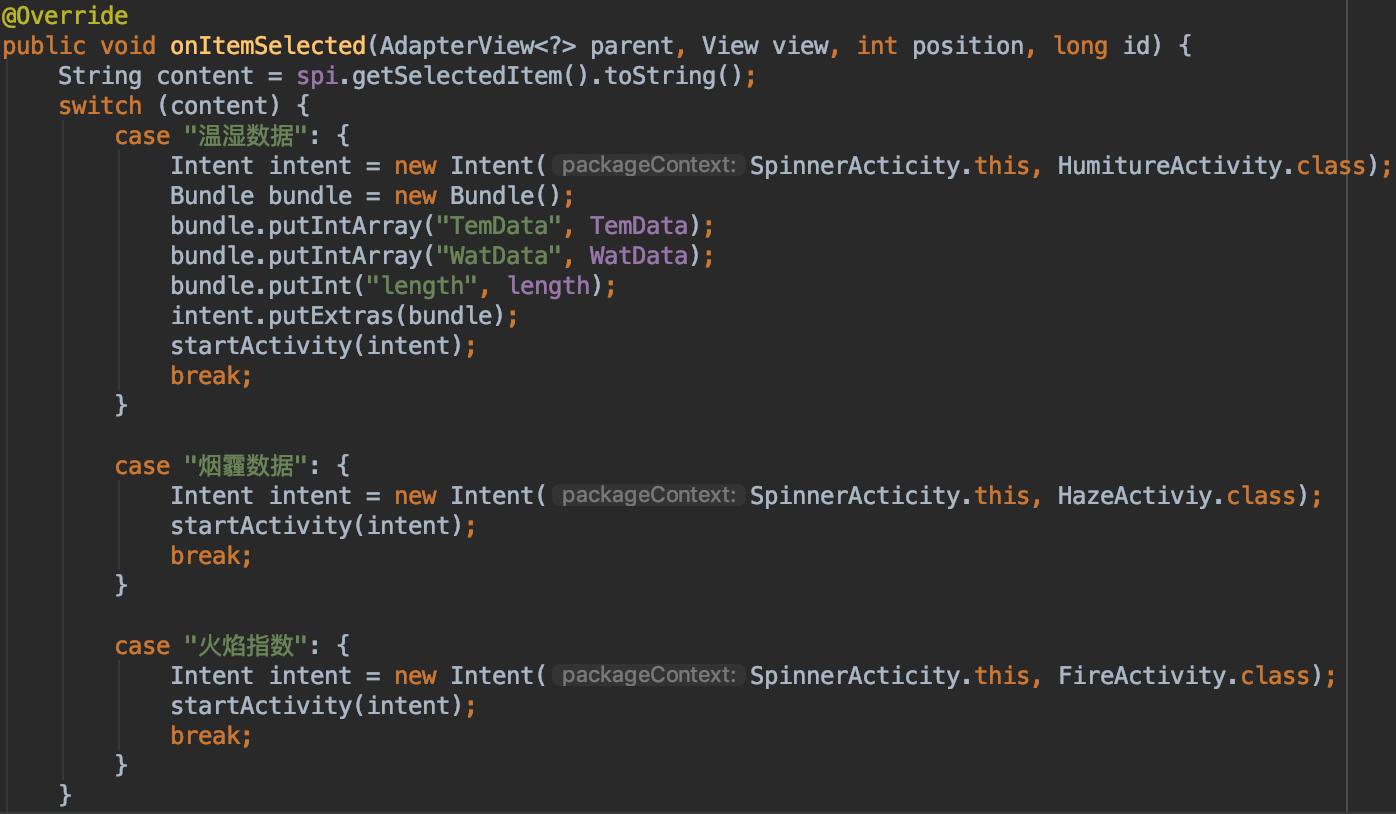
\includegraphics[width=0.8\textwidth]{figures/code/6}
    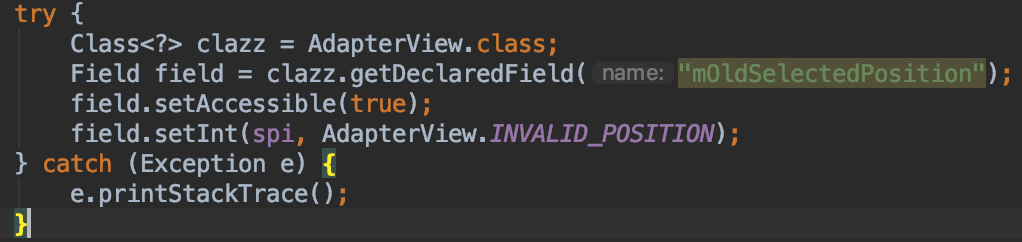
\includegraphics[width=0.8\textwidth]{figures/code/7}
    \caption{页面跳转}
\end{figure}

\item {APP与ESP8266建立TCP连接以及数据传输接受实现}:

通过监听连接Button的点击情况,使用线程以及socket传输与局域网服务器建立连接,ESP8266方面通过WIFI模块进行相同局域网连接,建立与APP之间的通讯。

\begin{figure}[htbp]
    \centering
    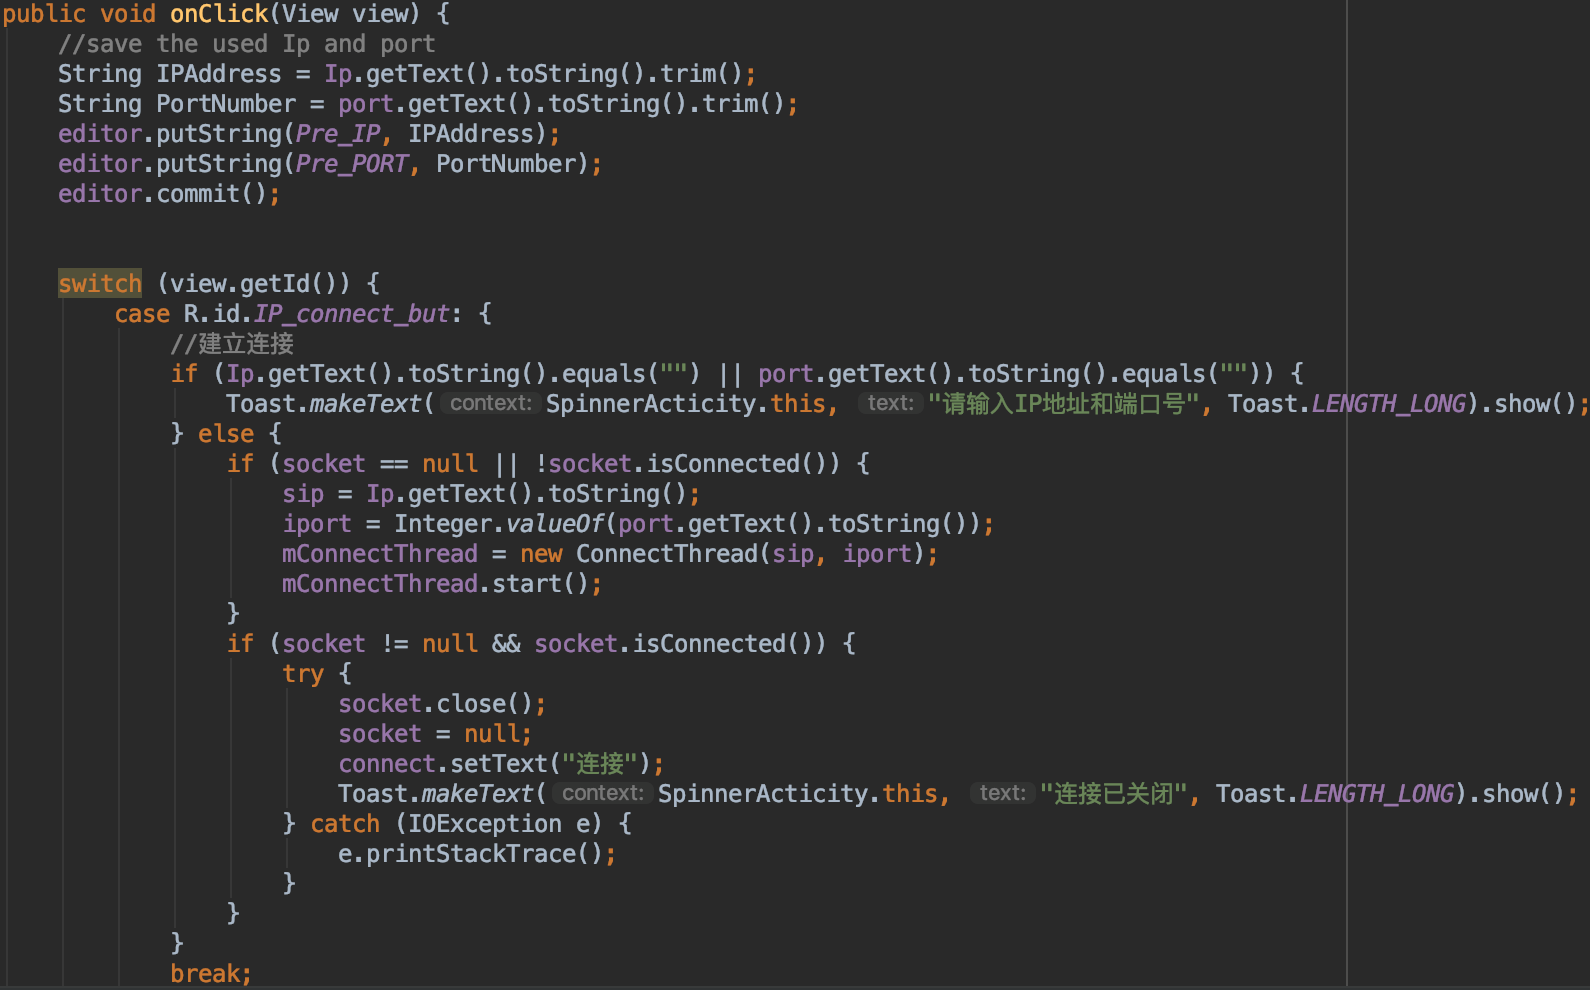
\includegraphics[width=0.8\textwidth]{figures/code/8}
    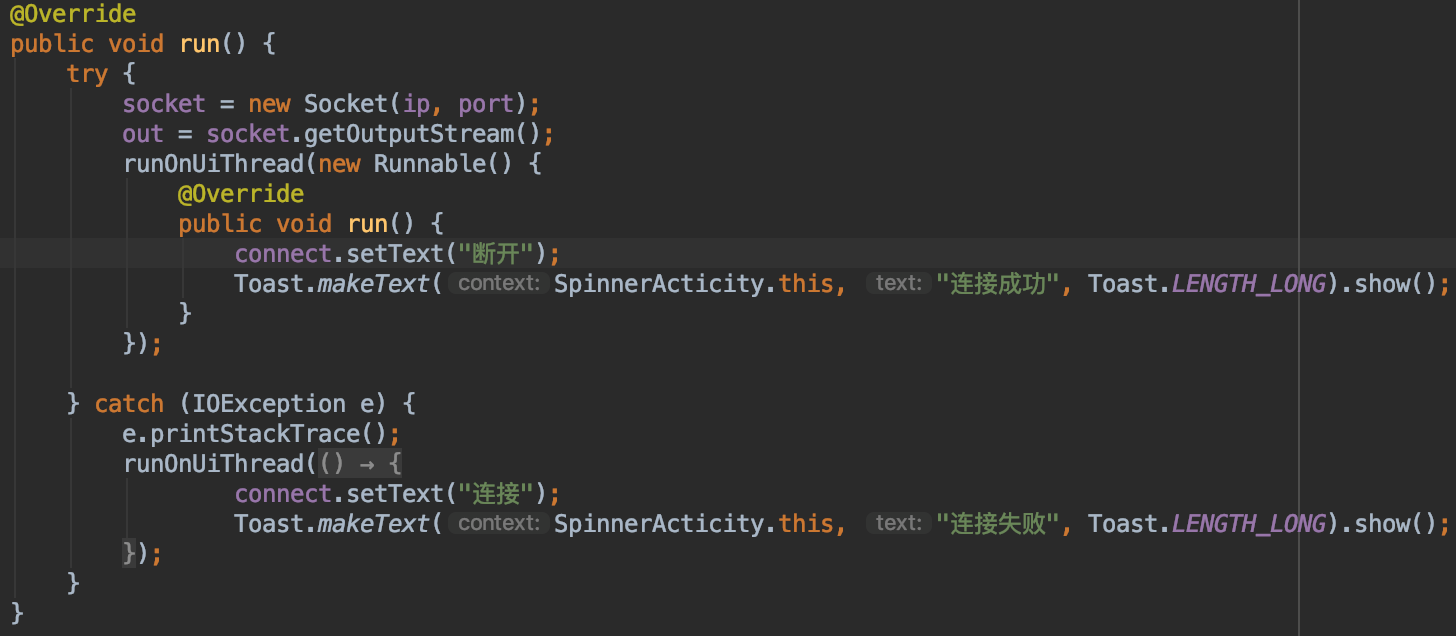
\includegraphics[width=0.8\textwidth]{figures/code/9}
    \caption{TCP协议通信}
\end{figure}

值得注意的是为防止切换界面后导致已输入的IP地址以及端口号清空,连接别打断,特使用了SharedPreferences.Editor来保存记录其连接情况。

传输数据使用的方法是socket的getOutputStream.write,可向服务器发送数据,并在服务器端接收响应回复相应动作,如开关灯即通过按钮监听动作向服务器发送请求数据。

\begin{figure}[htbp]
    \centering
    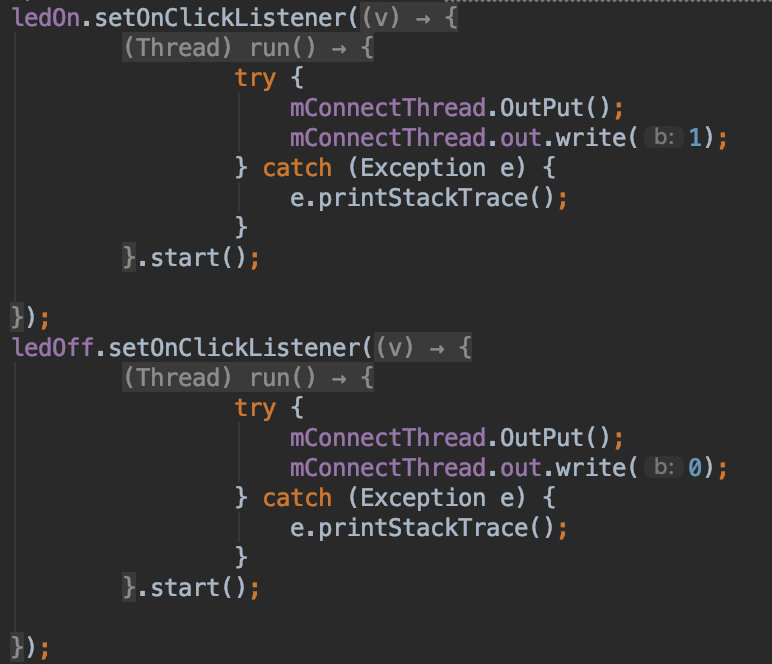
\includegraphics[width=0.8\textwidth]{figures/code/10}
    \caption{监听器}
\end{figure}

接受数据使用方式为客户端app向服务器发送请求数据,服务器返回数据给客户端,客户端调用接受线程ReceiveThread进行解析并接受存储,因温湿度时刻在改变所以使用timer计时器每隔一段时间请求一次数据进行更新。(此步与小组成员石琦合作完成)

\begin{figure}[htbp]
    \centering
    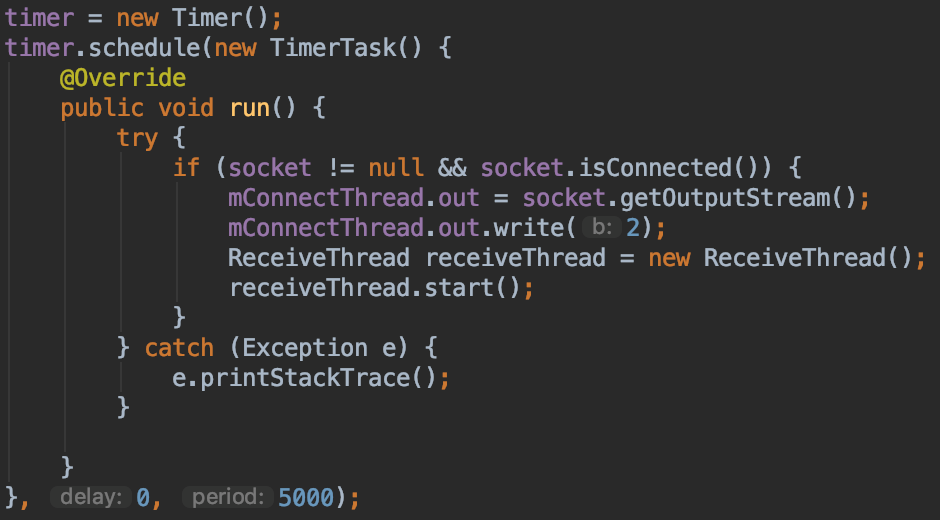
\includegraphics[width=0.8\textwidth]{figures/code/11}
    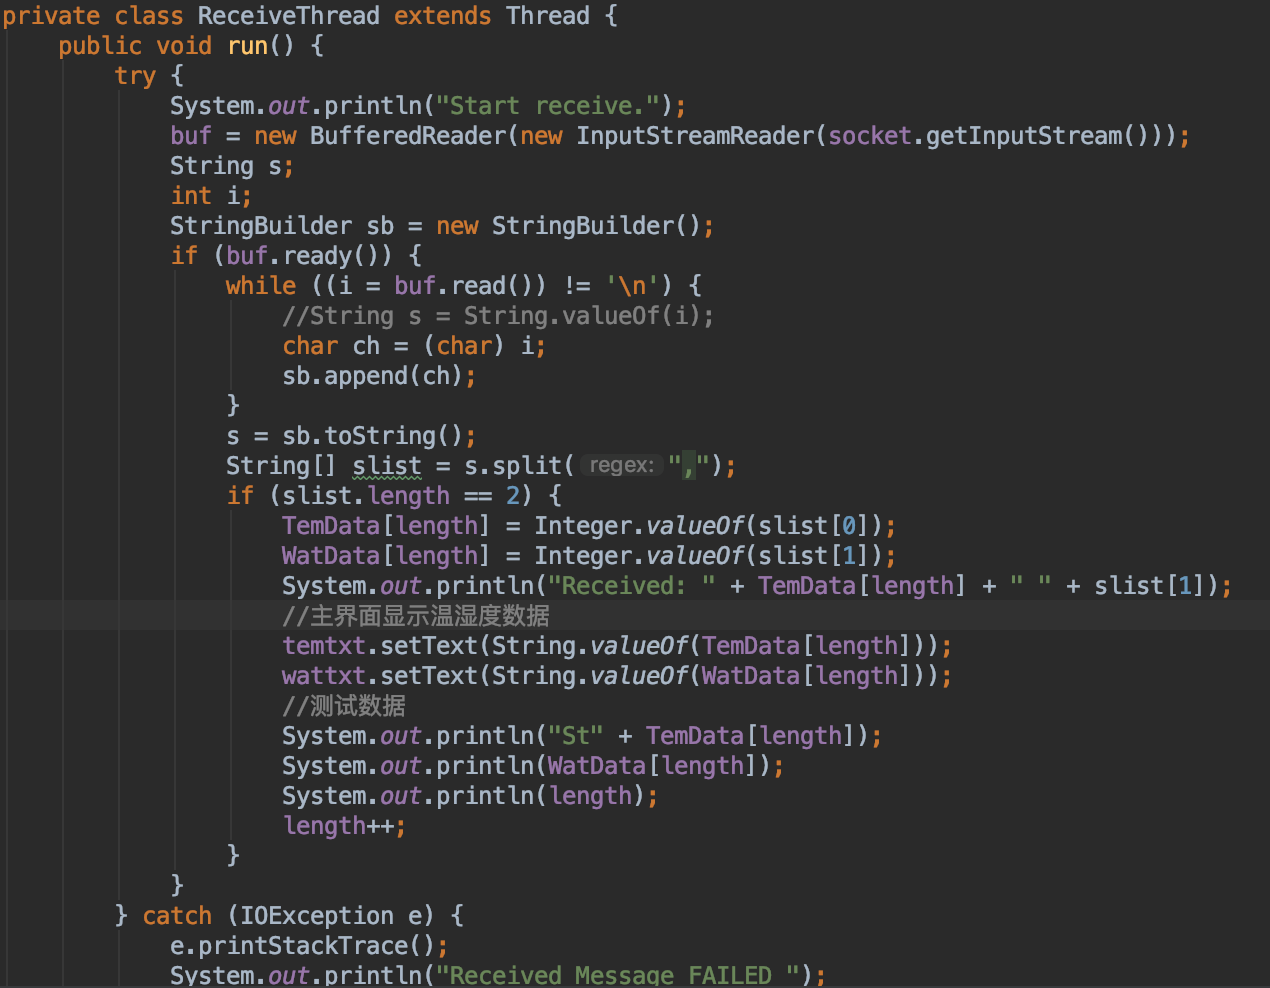
\includegraphics[width=0.8\textwidth]{figures/code/12}
    \caption{计时器和线程ReceiveThread}
\end{figure}

\item {历史数据折线图的绘制}:

首先设置数组通过Bundle和getIntent接受主界面传输回的数据,然后通过HelloChart中的组件先设置数据点的集合,然后设置两条不同的线分别代表不同数据传入到线集合中。

\begin{figure}[htbp]
    \centering
    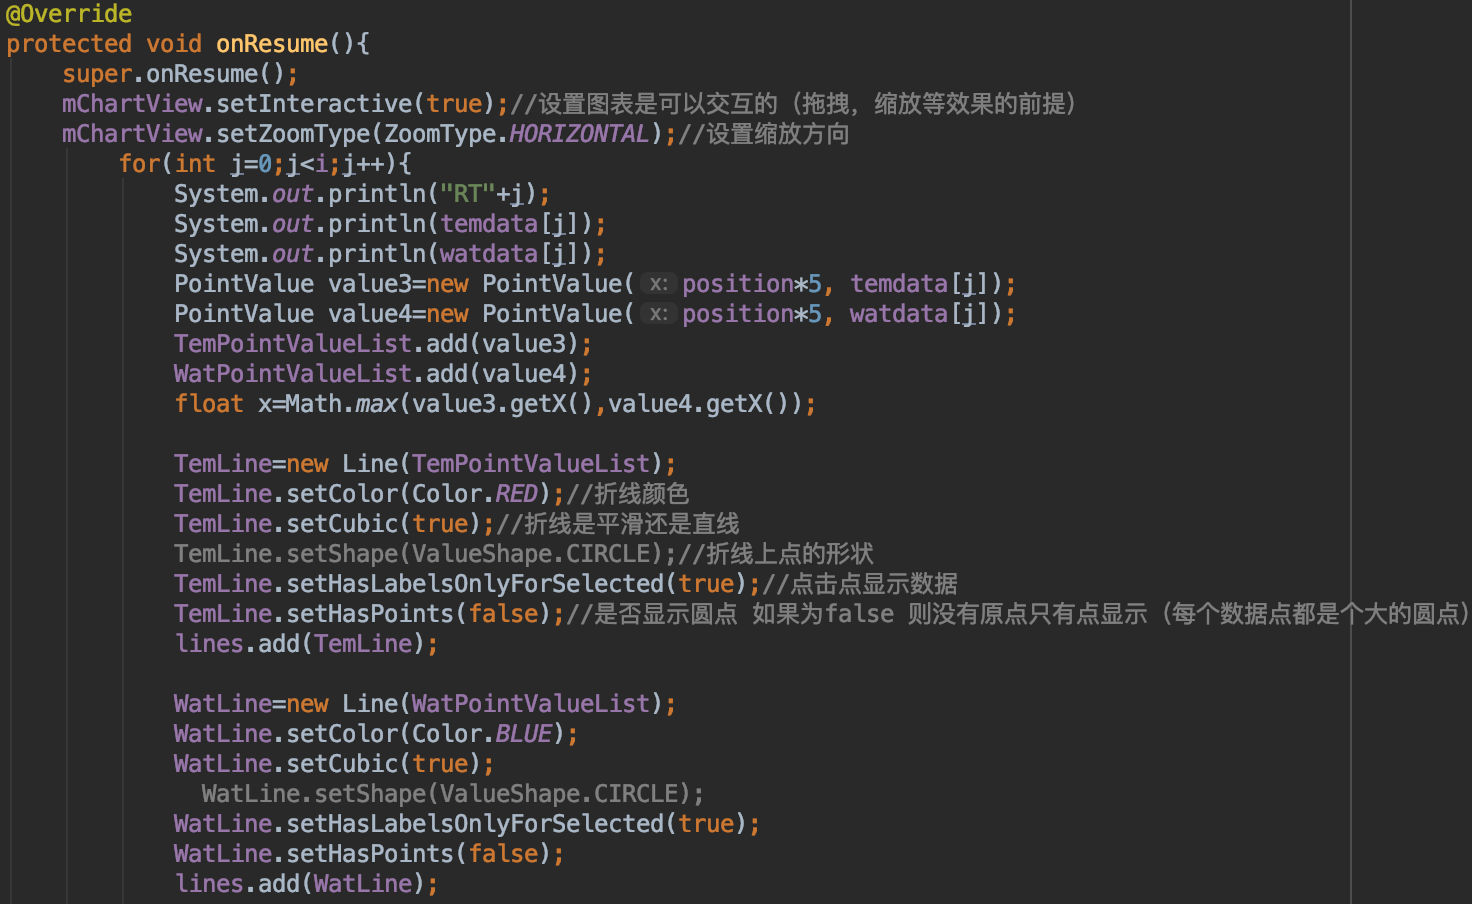
\includegraphics[width=0.8\textwidth]{figures/code/13}
\end{figure}

使用函数initData建立坐标轴X,Y,并建立函数设置坐标图的最大数据显示范围以及当前数据显示区域。可根据当前数据情况进行折线图的动态移动,为折线图设置属性setInteractive以及setZoomType可以对折线图进行拖动查看。

\begin{figure}[htbp]
    \centering
    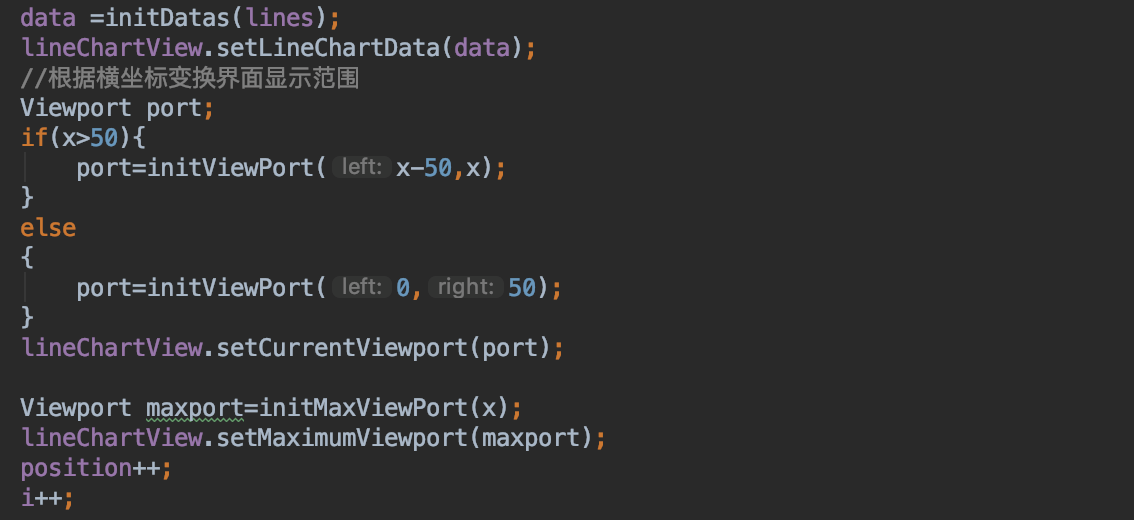
\includegraphics[width=0.8\textwidth]{figures/code/14}
    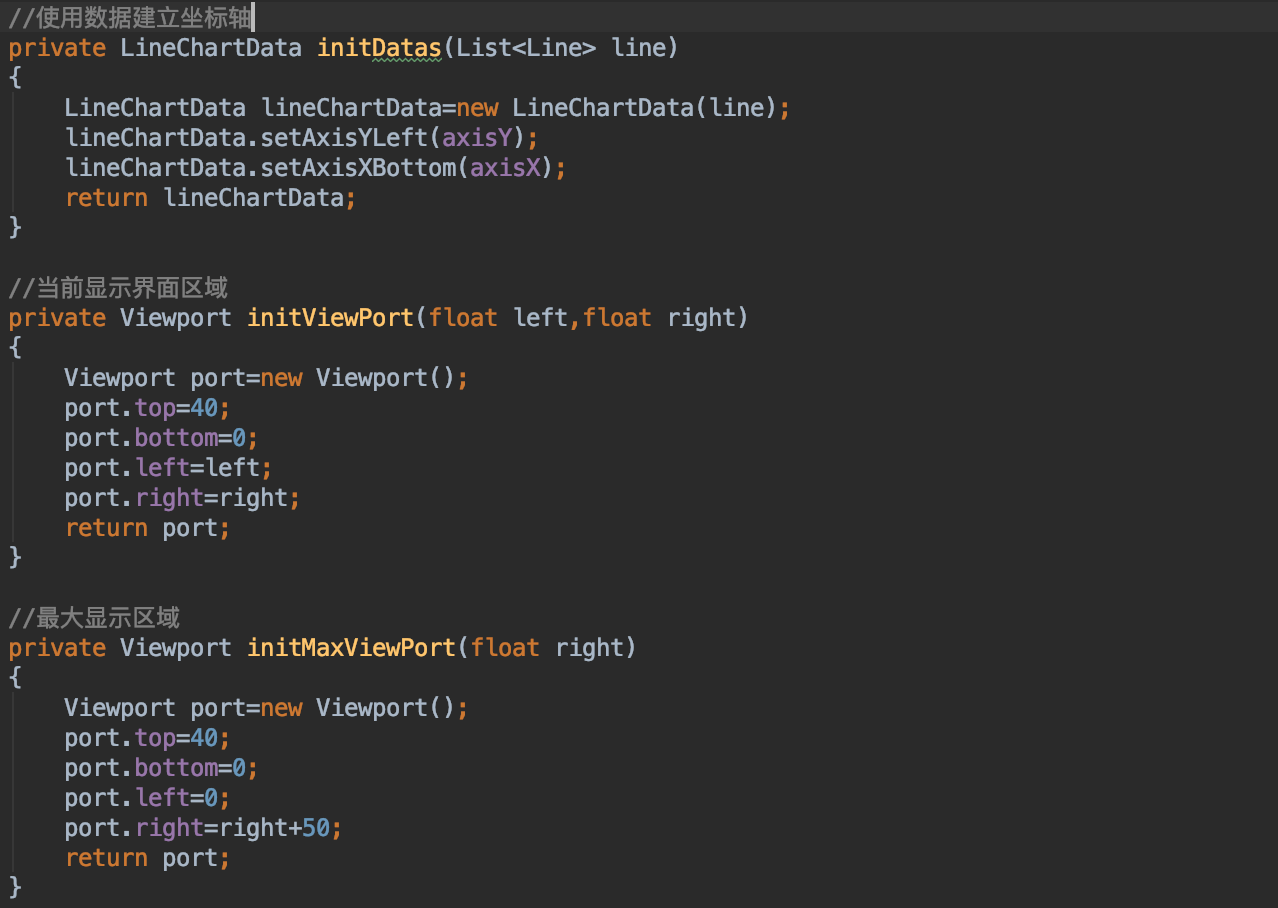
\includegraphics[width=0.8\textwidth]{figures/code/15}
\end{figure}

函数PrintHumitureLine进行对坐标轴X,Y的属性设置以及折线图行为属性的设置,开始使用数据进行进行绘图。

\begin{figure}[htbp]
    \centering
    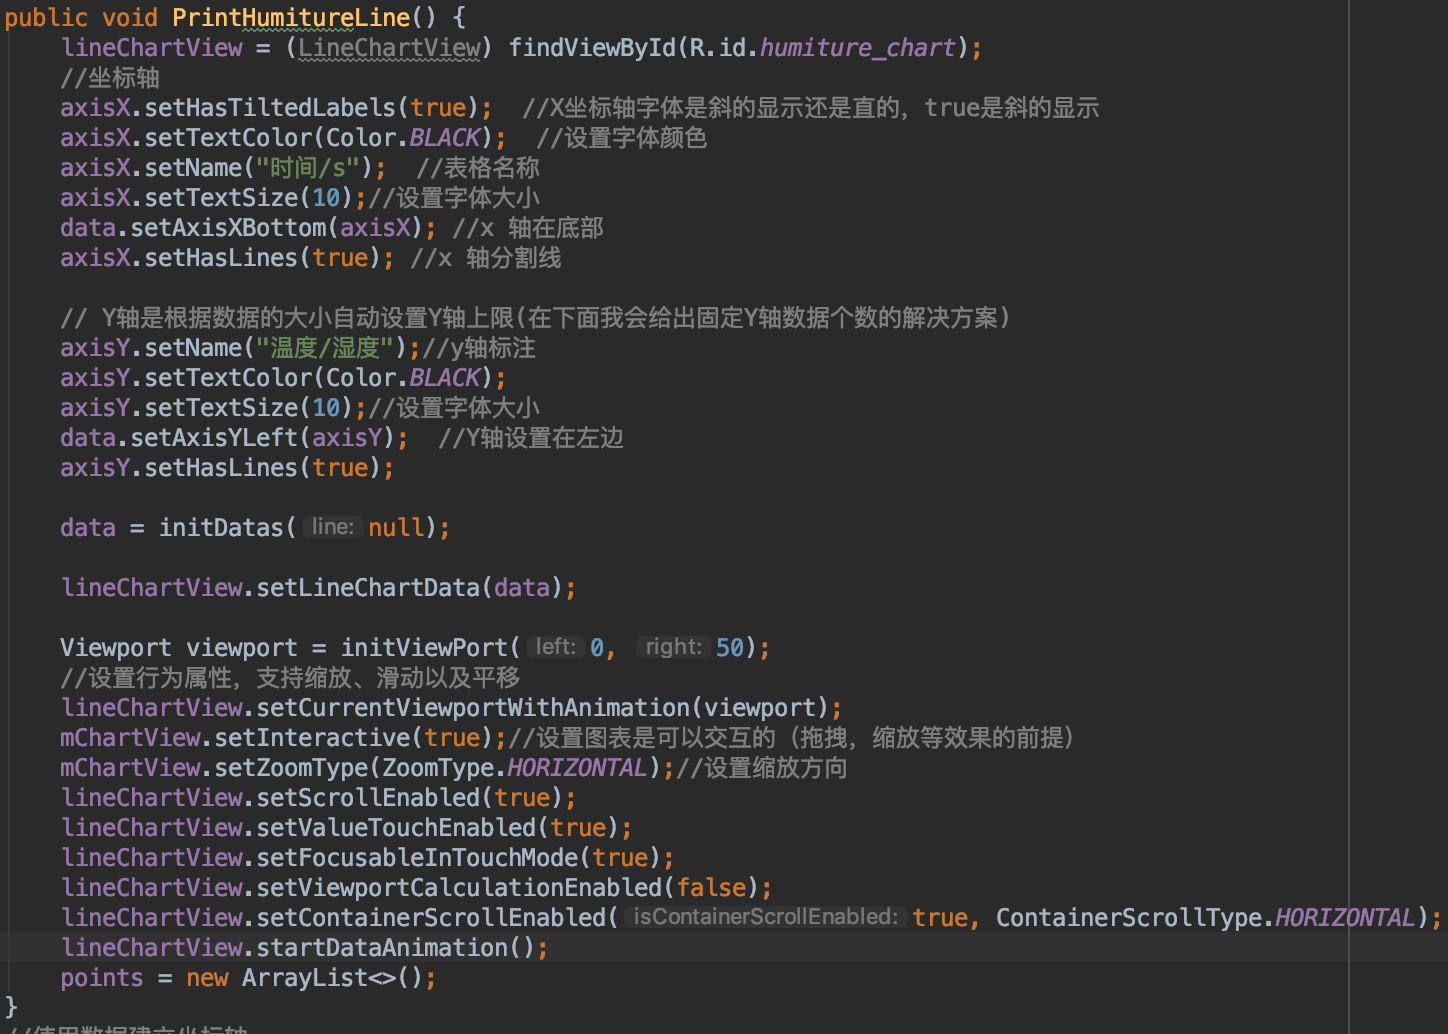
\includegraphics[width=0.8\textwidth]{figures/code/16}
\end{figure}

\end{enumerate}

\section{Web页面设计及数据通信}

考虑到需求的功能主要有控制LED灯的开关、检测室内温湿度、检测烟雾、检测火焰四个方面,并且与APP相照应,故而将网页设计为主页、LED灯、温湿数据、烟霾数据、火焰指数五个页面,并为五个页面设计导航栏。

在主页中,添加一个slider用来动态显示几个传感器的图片,增加页面美感。同时在下方显示所有数据并实时自动更新。自动刷新数据使用setInterval(function, time)定时调用。获取数据使用XMLHttpRequest()方法,并在单片机中烧录相关响应代码,即使用webServer.on()方法接收请求,用webServer.send()方法发送响应,主要代码如下:

\begin{figure}[htbp]
    \centering
    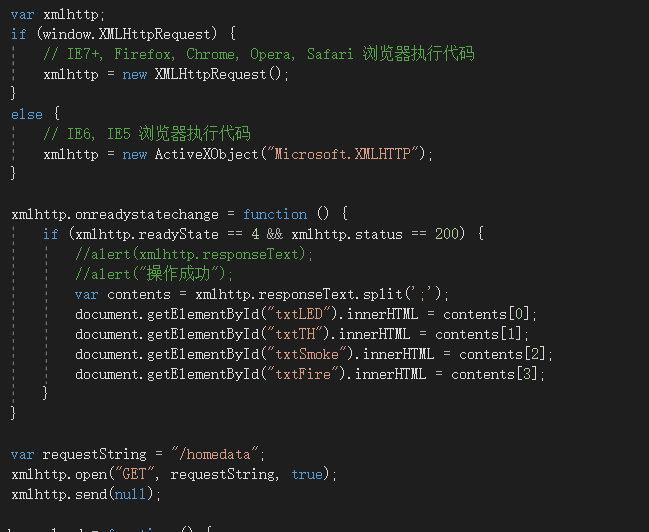
\includegraphics[width=0.8\textwidth]{figures/code/4}
    \caption{使用XMLHttpRequest()方法与服务器通信}
\end{figure}

LED页面实时监听LED灯的开关状态,并随之改变img的src属性,使之实现开关灯的图片效果,仍然使用http的方式与服务区通信。

温湿数据页面同样用定时器实时显示室内温湿度数据,除此之外,还使用jQuery+Highcharts包绘制温湿度历史数据折线图,每五秒刷新一次数据,增加一条折线。实现代码如下:

\begin{figure}[htbp]
    \centering
    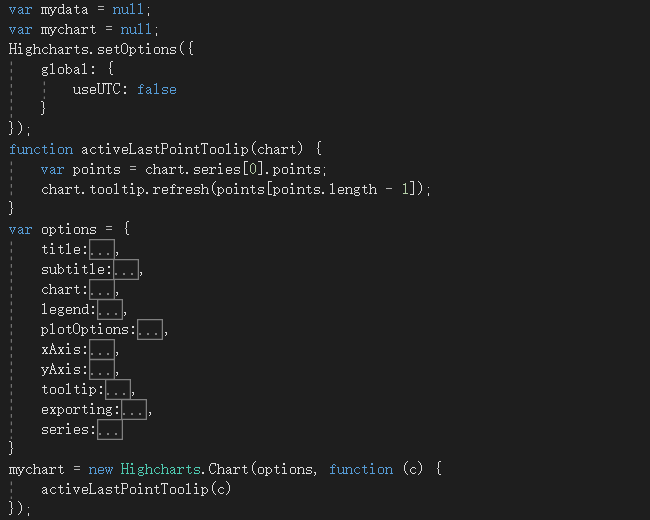
\includegraphics[width=0.8\textwidth]{figures/code/5}
    \caption{Highcharts折线图的属性}
\end{figure}

烟霾指数页面和火焰指数页面用定时器实时刷新服务器端的烟雾数据和火焰情况,并在出现火焰的时候在火焰指数界面使用alert()弹出警告提示框。
	% !Mode:: "TeX:UTF-8"

\chapter{测试情况}

\section{APP最终界面及测试结果}

APP界面最终样式如下图,各界面皆可成功跳转。

\begin{figure}[h]
    \centering
    \begin{minipage}{0.3\textwidth}
        \centering
        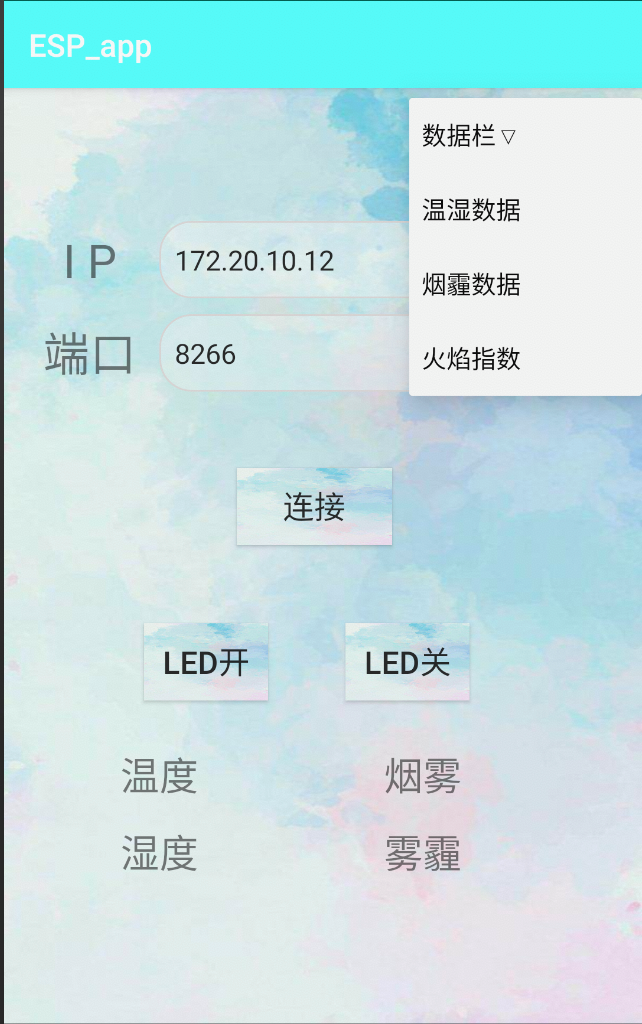
\includegraphics[width=0.9\textwidth]{figures/test/1}   
    \end{minipage}
    \begin{minipage}{0.3\textwidth}
        \centering
        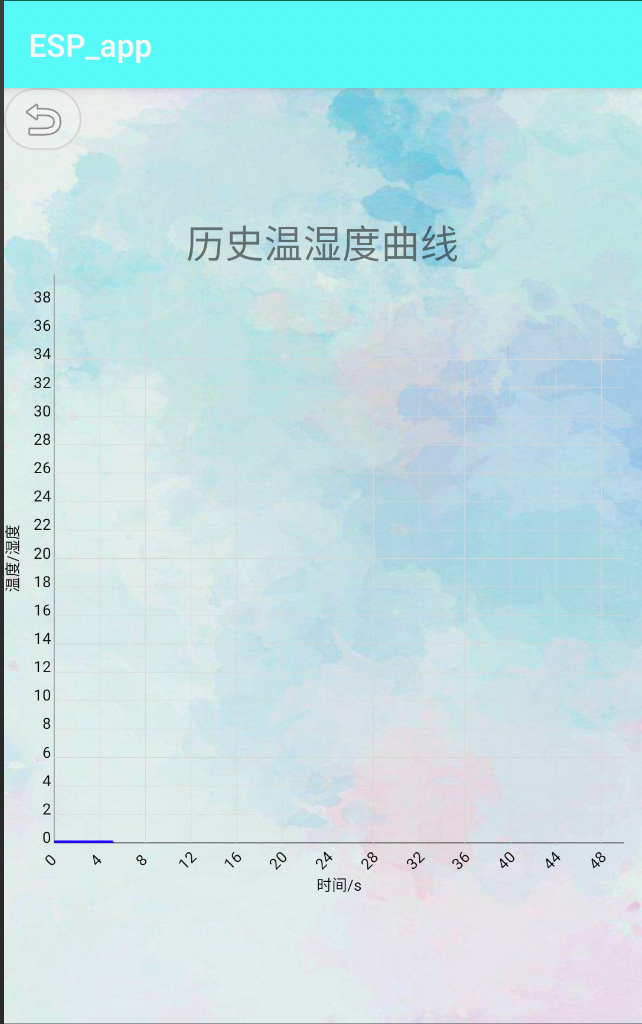
\includegraphics[width=0.9\textwidth]{figures/test/2}   
    \end{minipage}
    \begin{minipage}{0.3\textwidth}
        \centering
        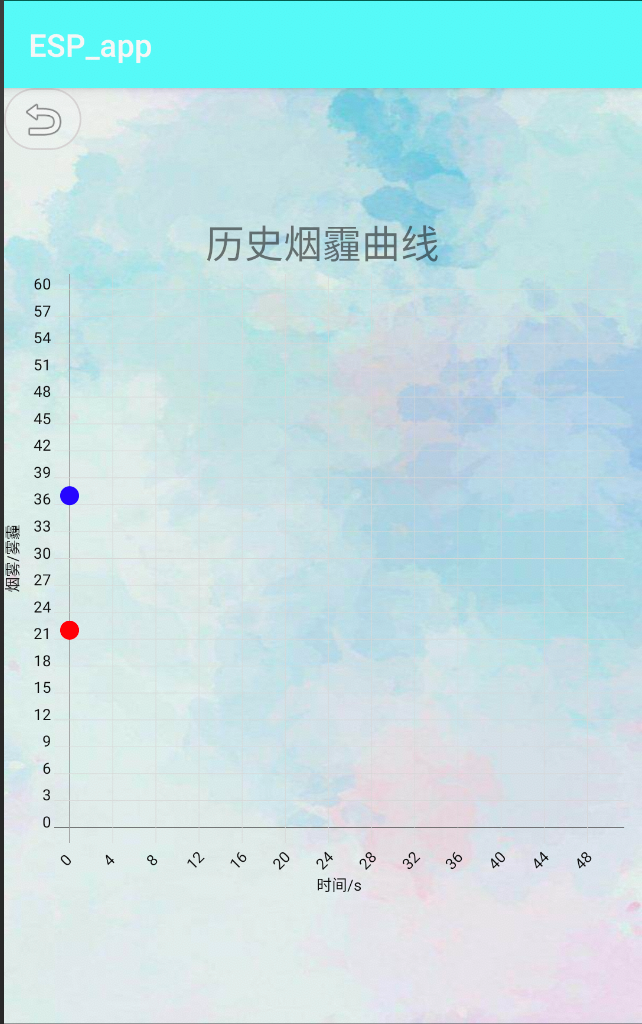
\includegraphics[width=0.9\textwidth]{figures/test/3}   
    \end{minipage}
\end{figure}

经测试,APP各数据接收正常,能成功绘制出温湿度历史曲线。

\section{Web最终界面及测试结果}

Web界面最终样式如下图,各页面均可成功切换。

\begin{figure}[h]
    \centering
    \begin{minipage}{0.4\textwidth}
        \centering
        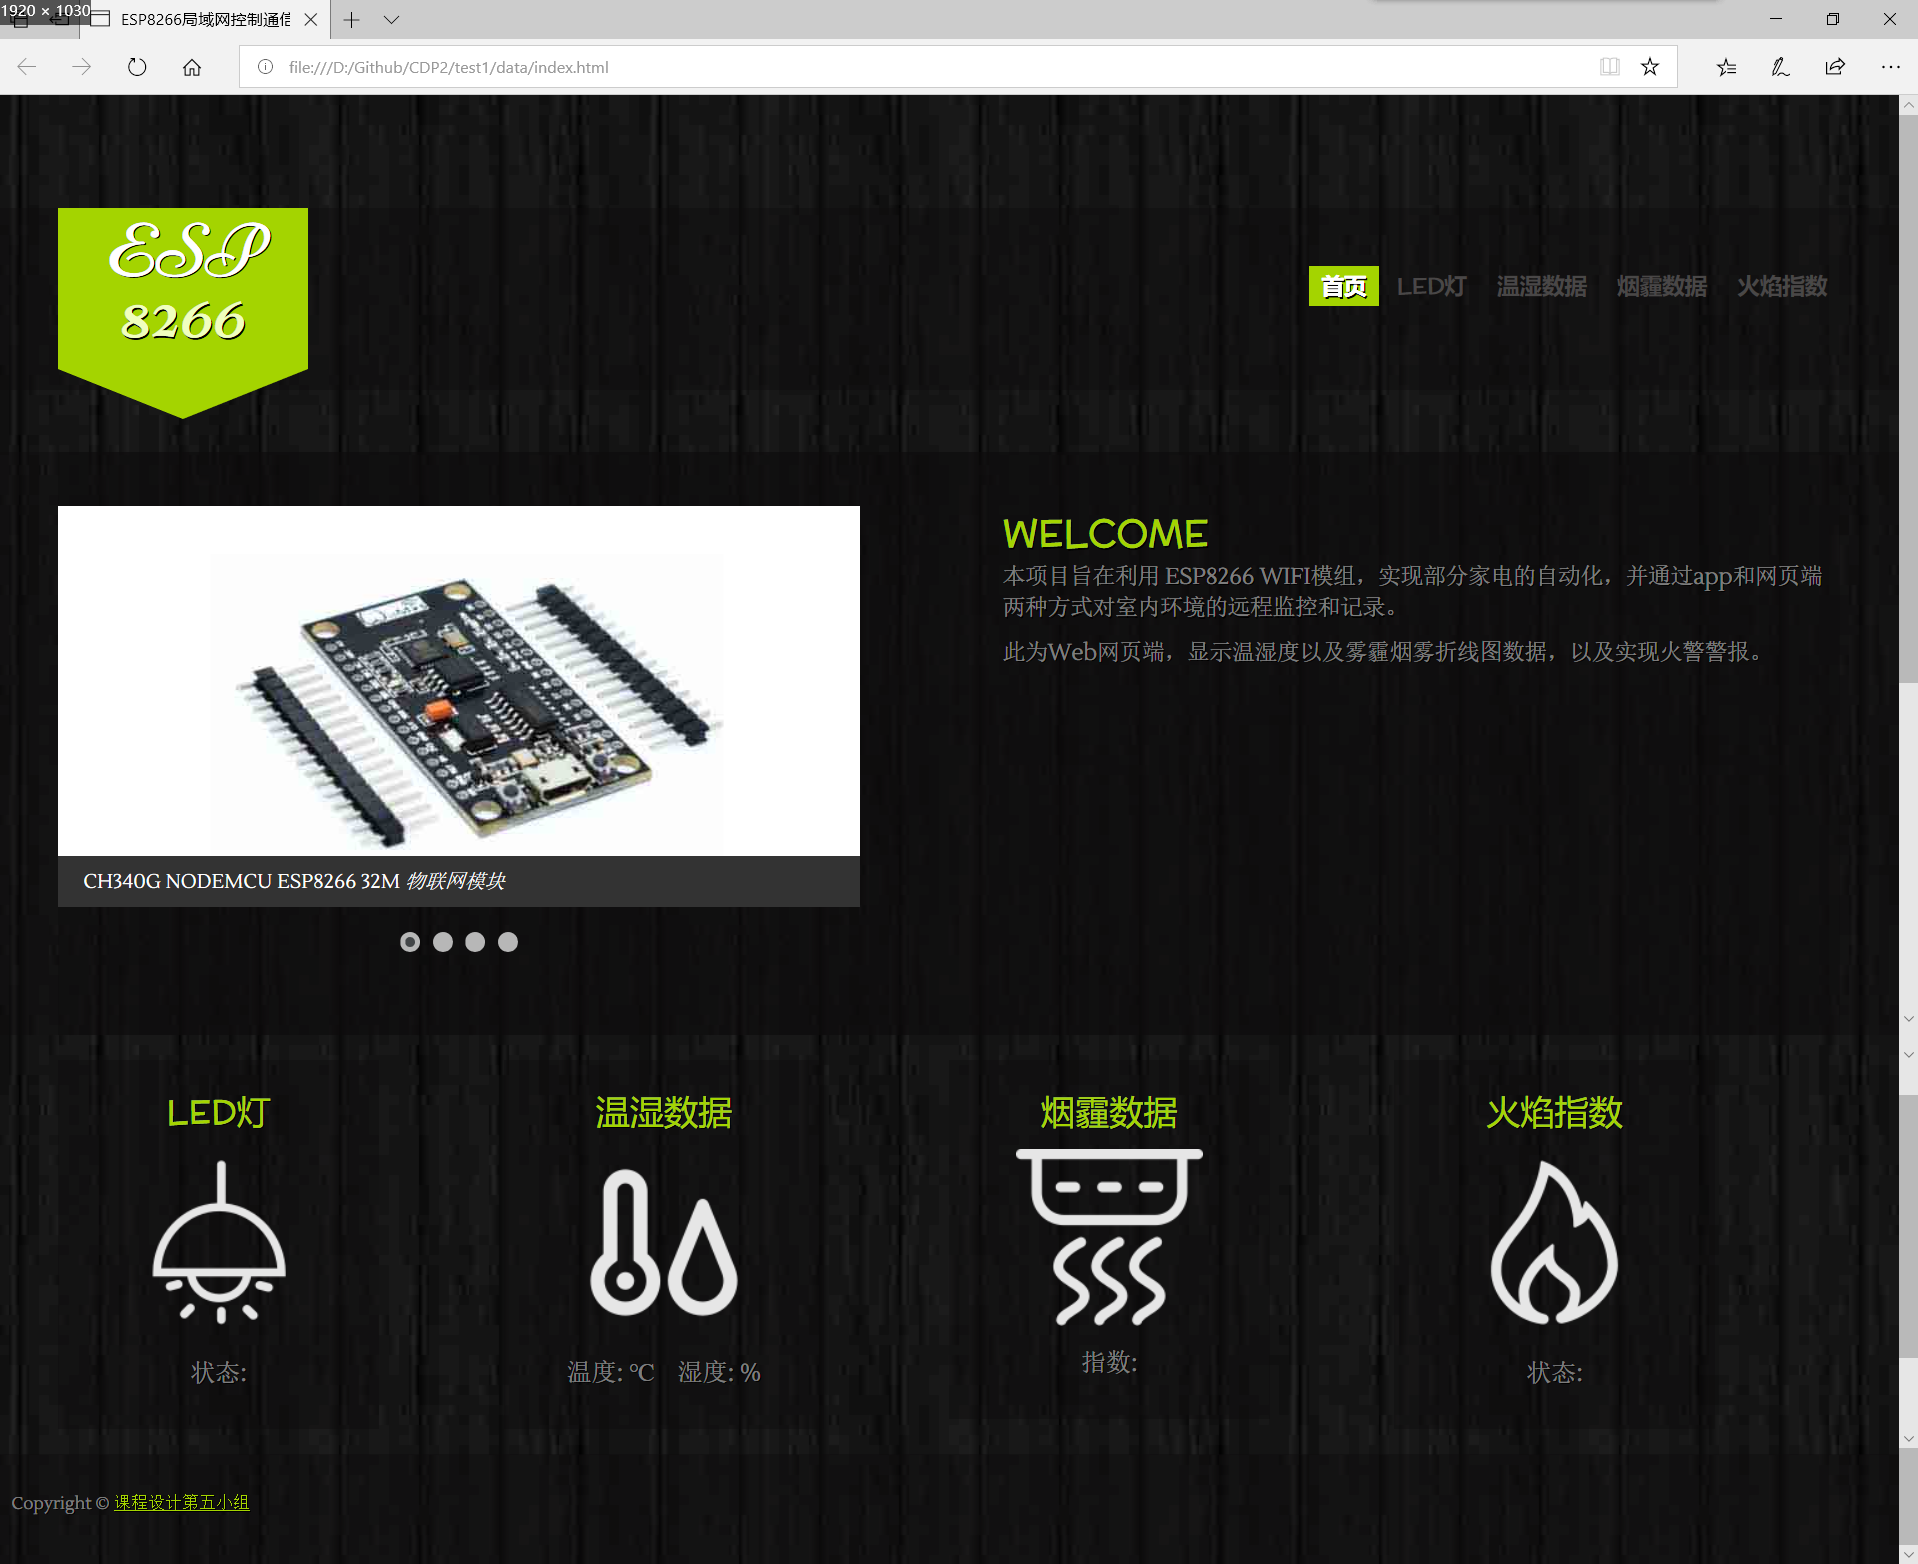
\includegraphics[width=0.7\textwidth]{figures/test/4}   
    \end{minipage}
    \begin{minipage}{0.4\textwidth}
        \centering
        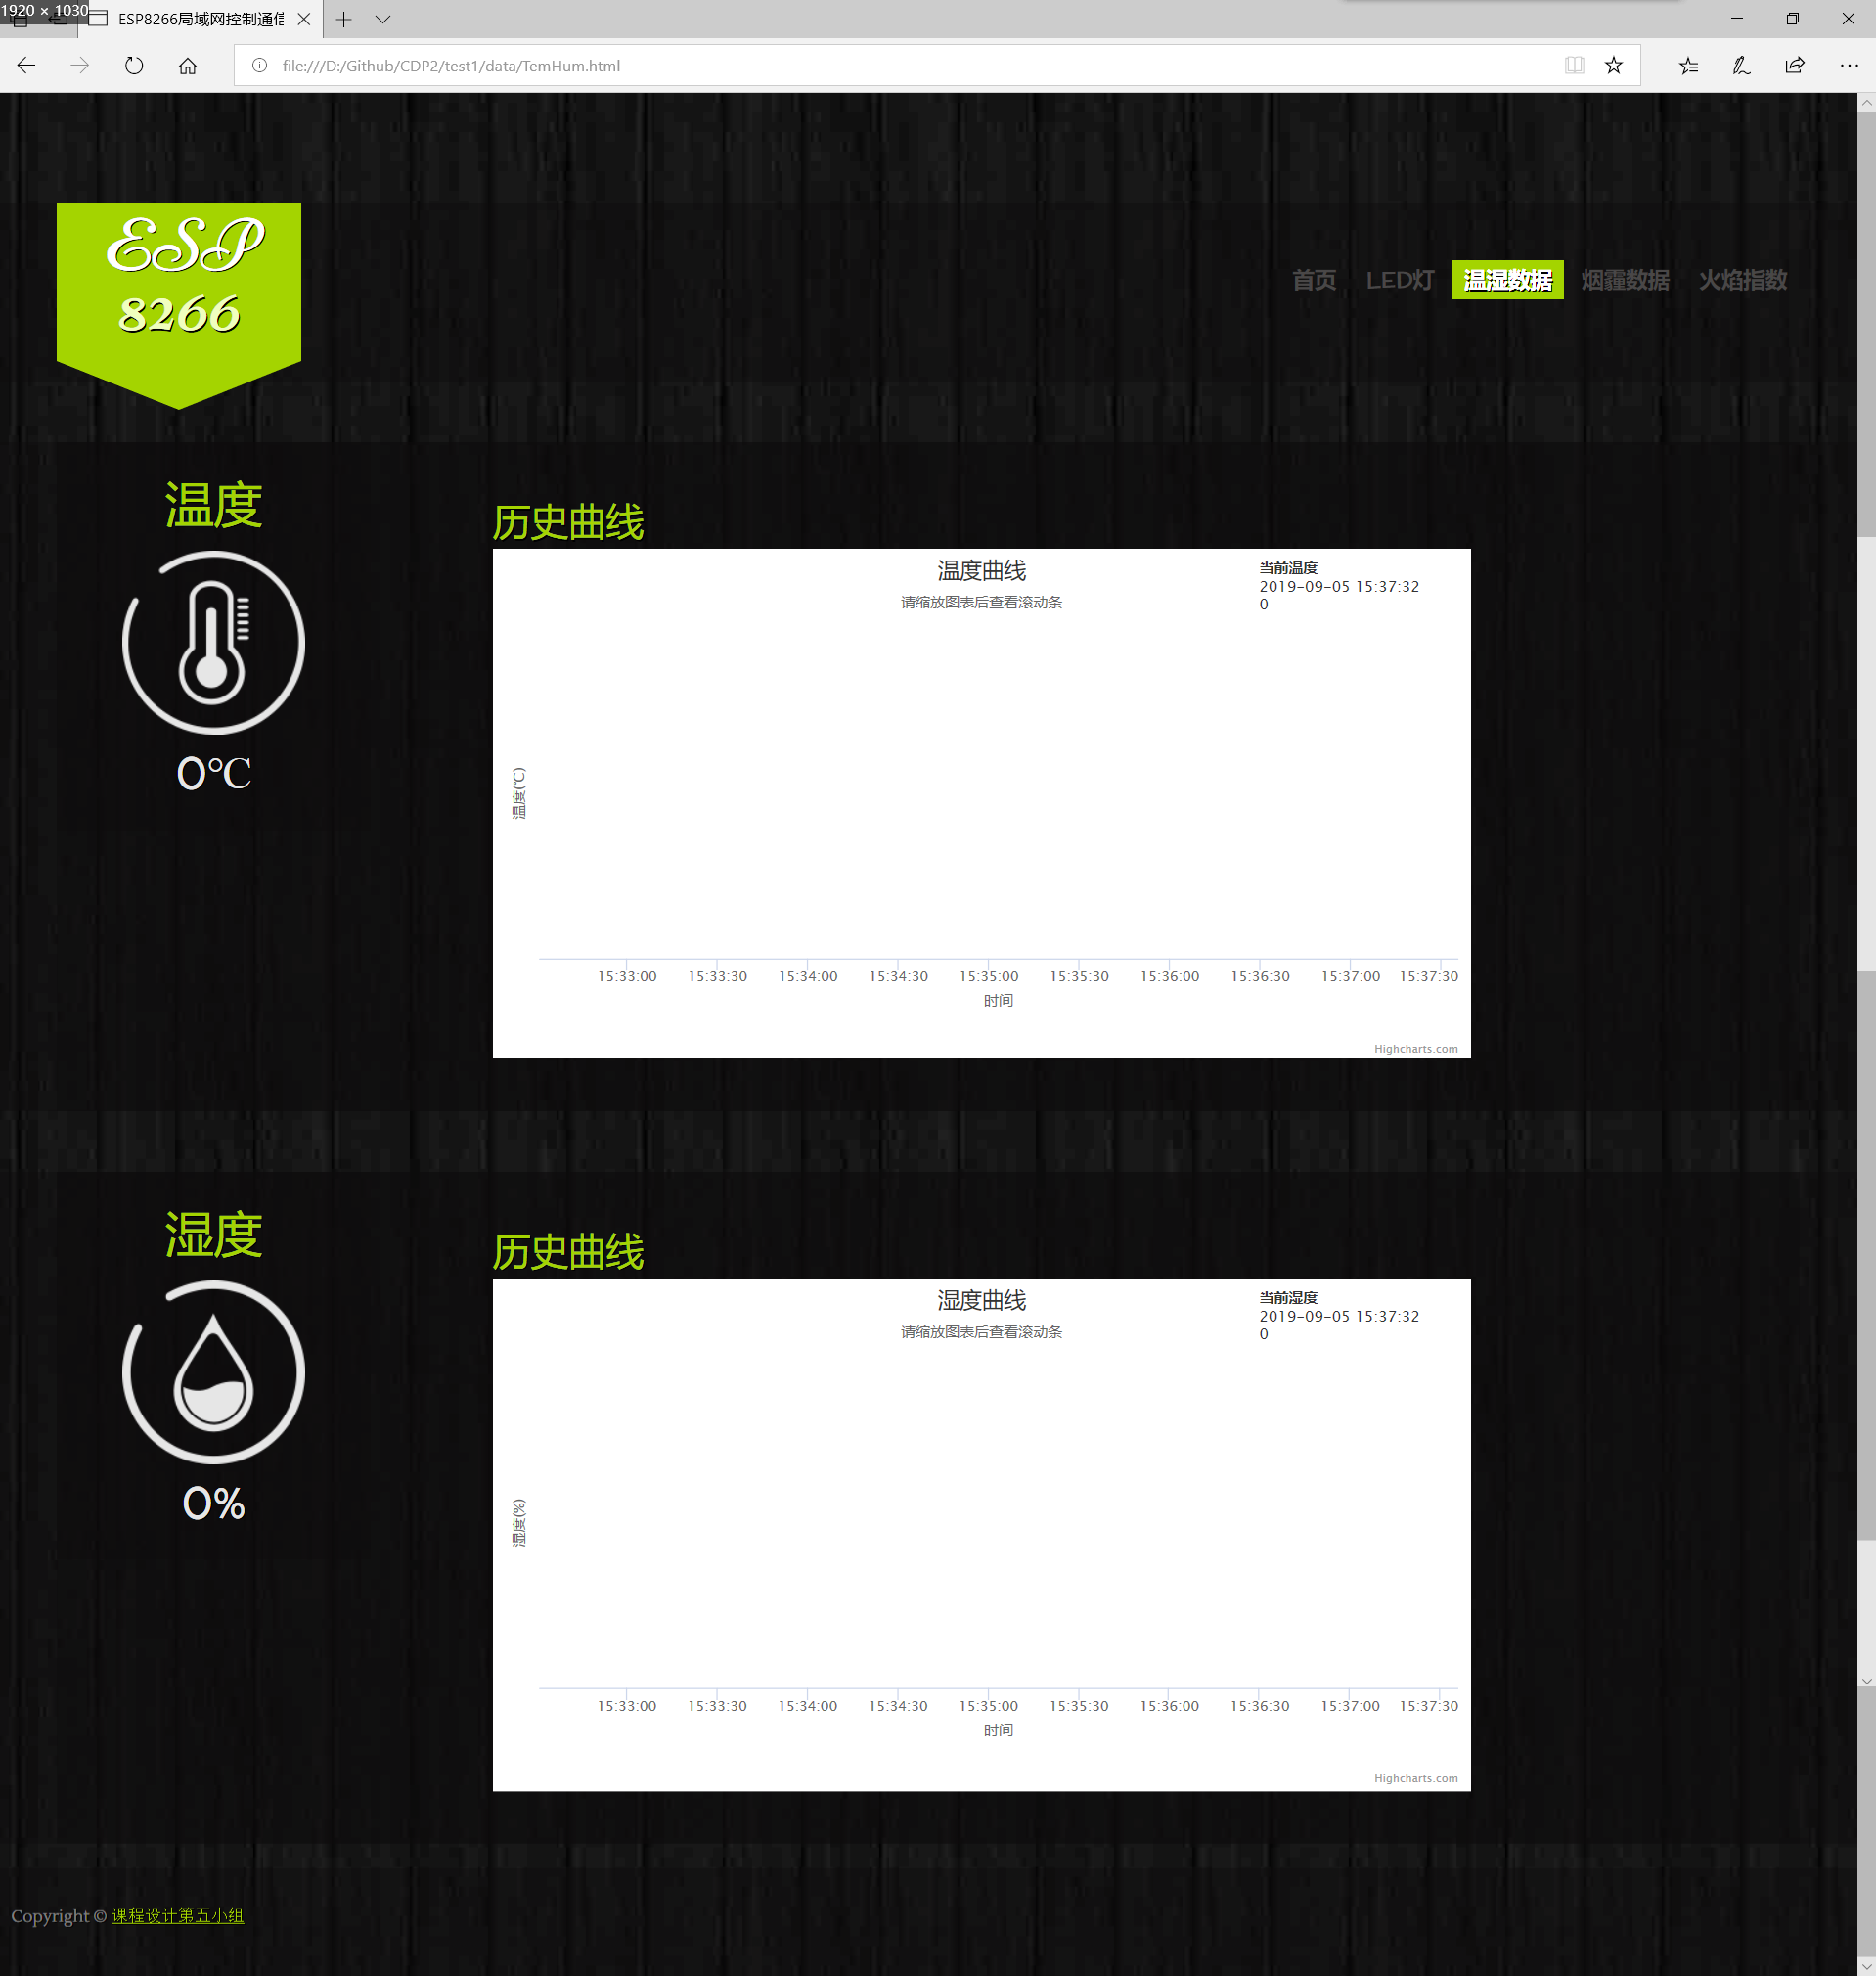
\includegraphics[width=0.7\textwidth]{figures/test/6}   
    \end{minipage}
    \vspace{\baselineskip} 
    
    \centering
    \begin{minipage}{0.3\textwidth}
        \centering
        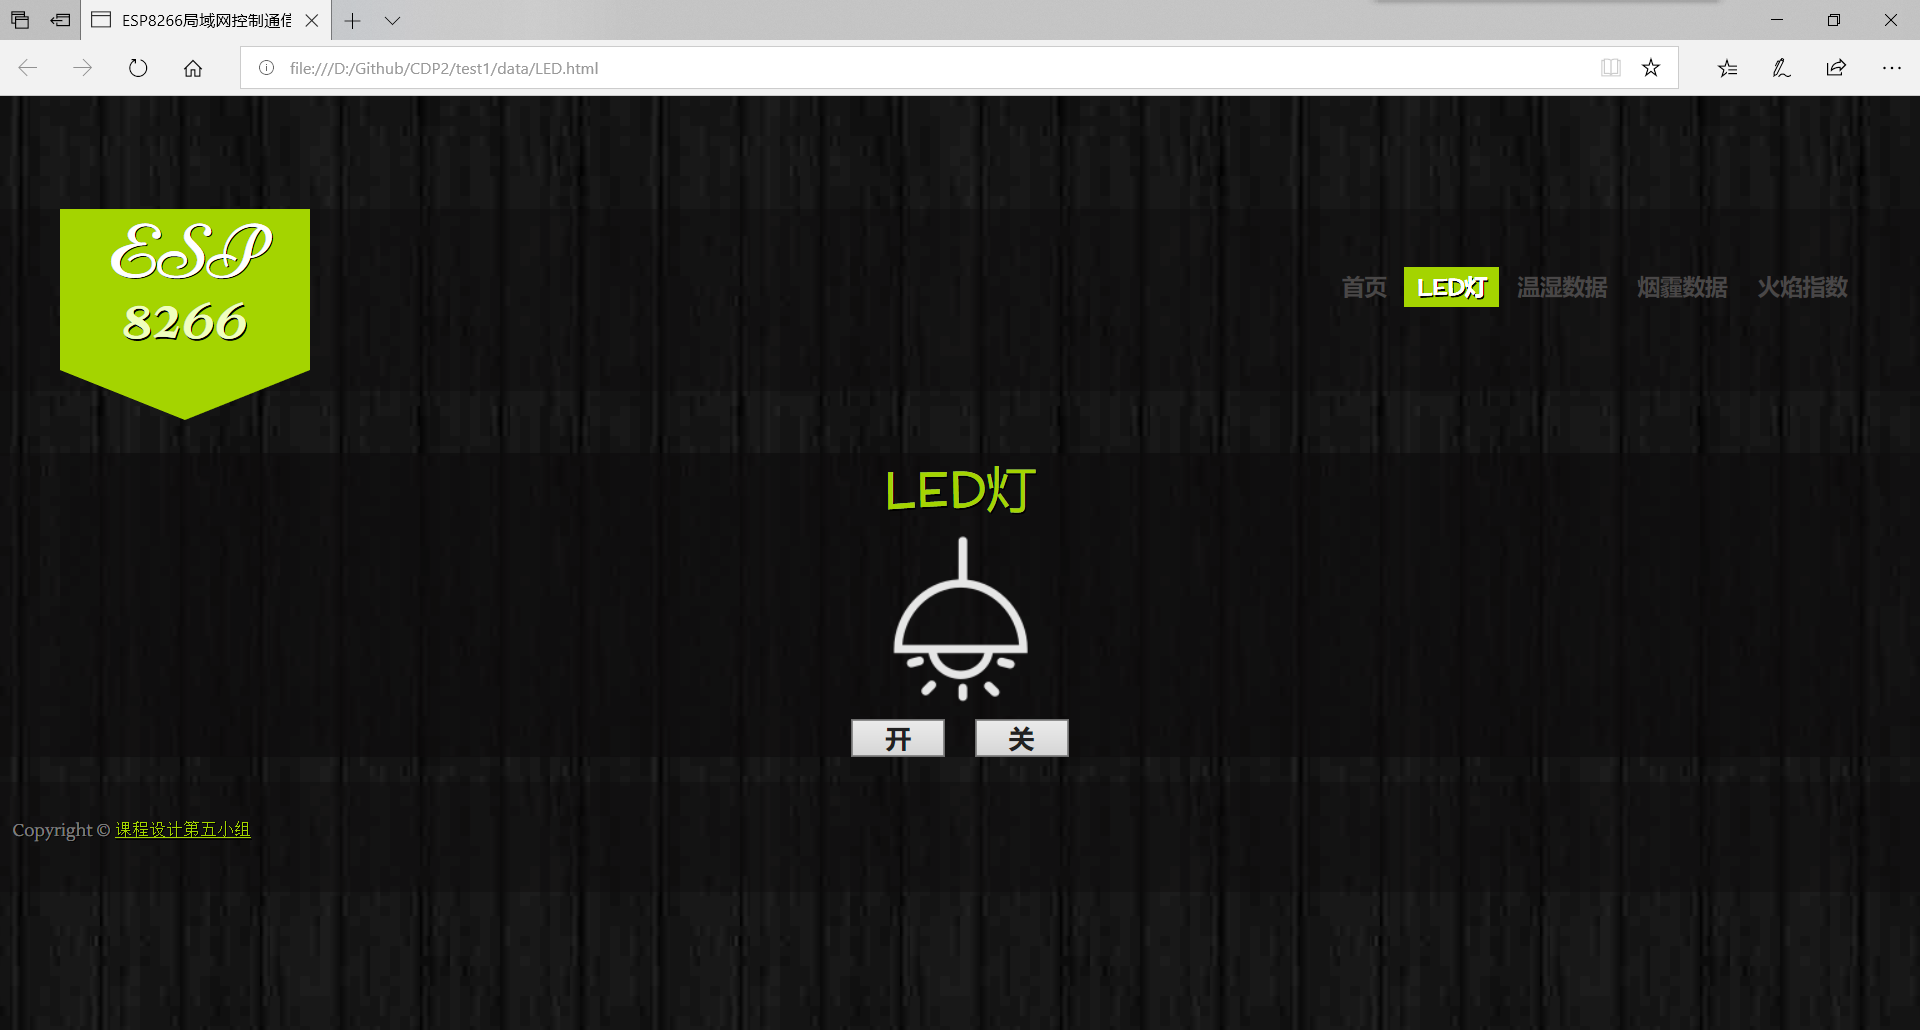
\includegraphics[width=0.95\textwidth]{figures/test/5}   
    \end{minipage}
    \begin{minipage}{0.3\textwidth}
        \centering
        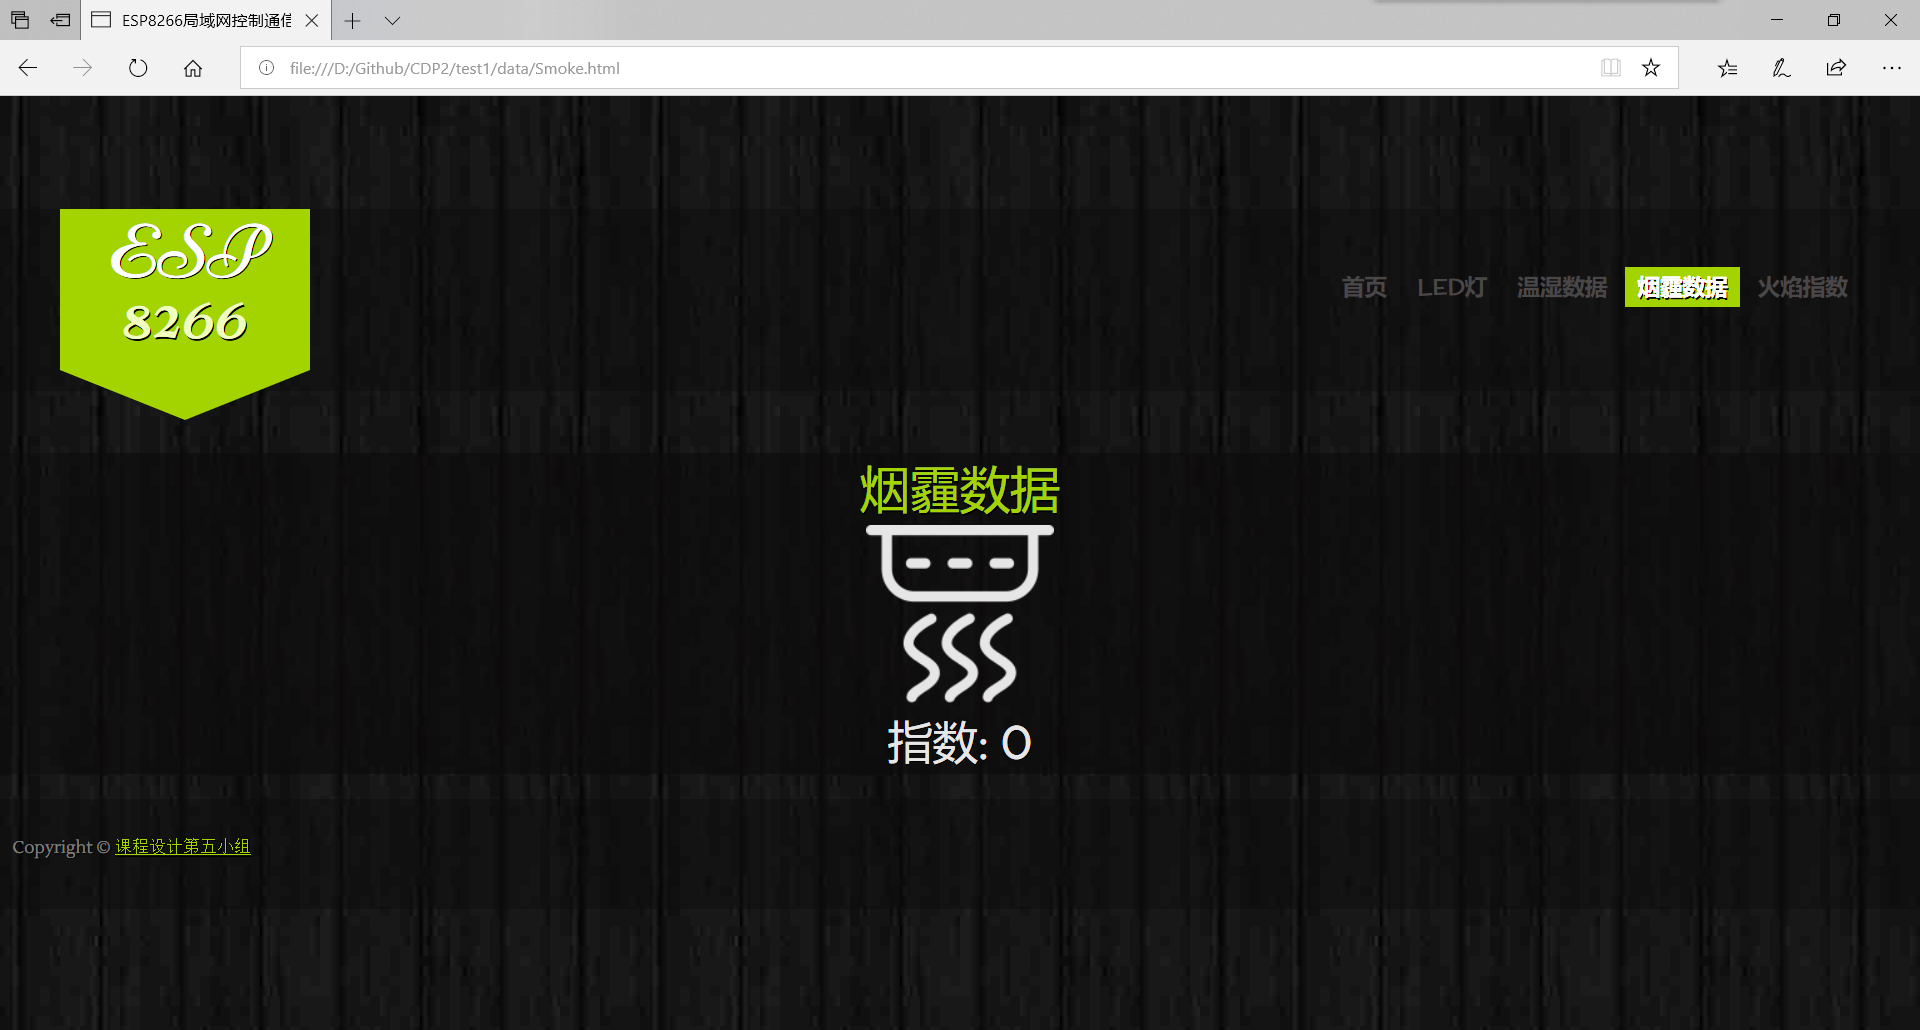
\includegraphics[width=0.95\textwidth]{figures/test/7}   
    \end{minipage}
    \begin{minipage}{0.3\textwidth}
        \centering
        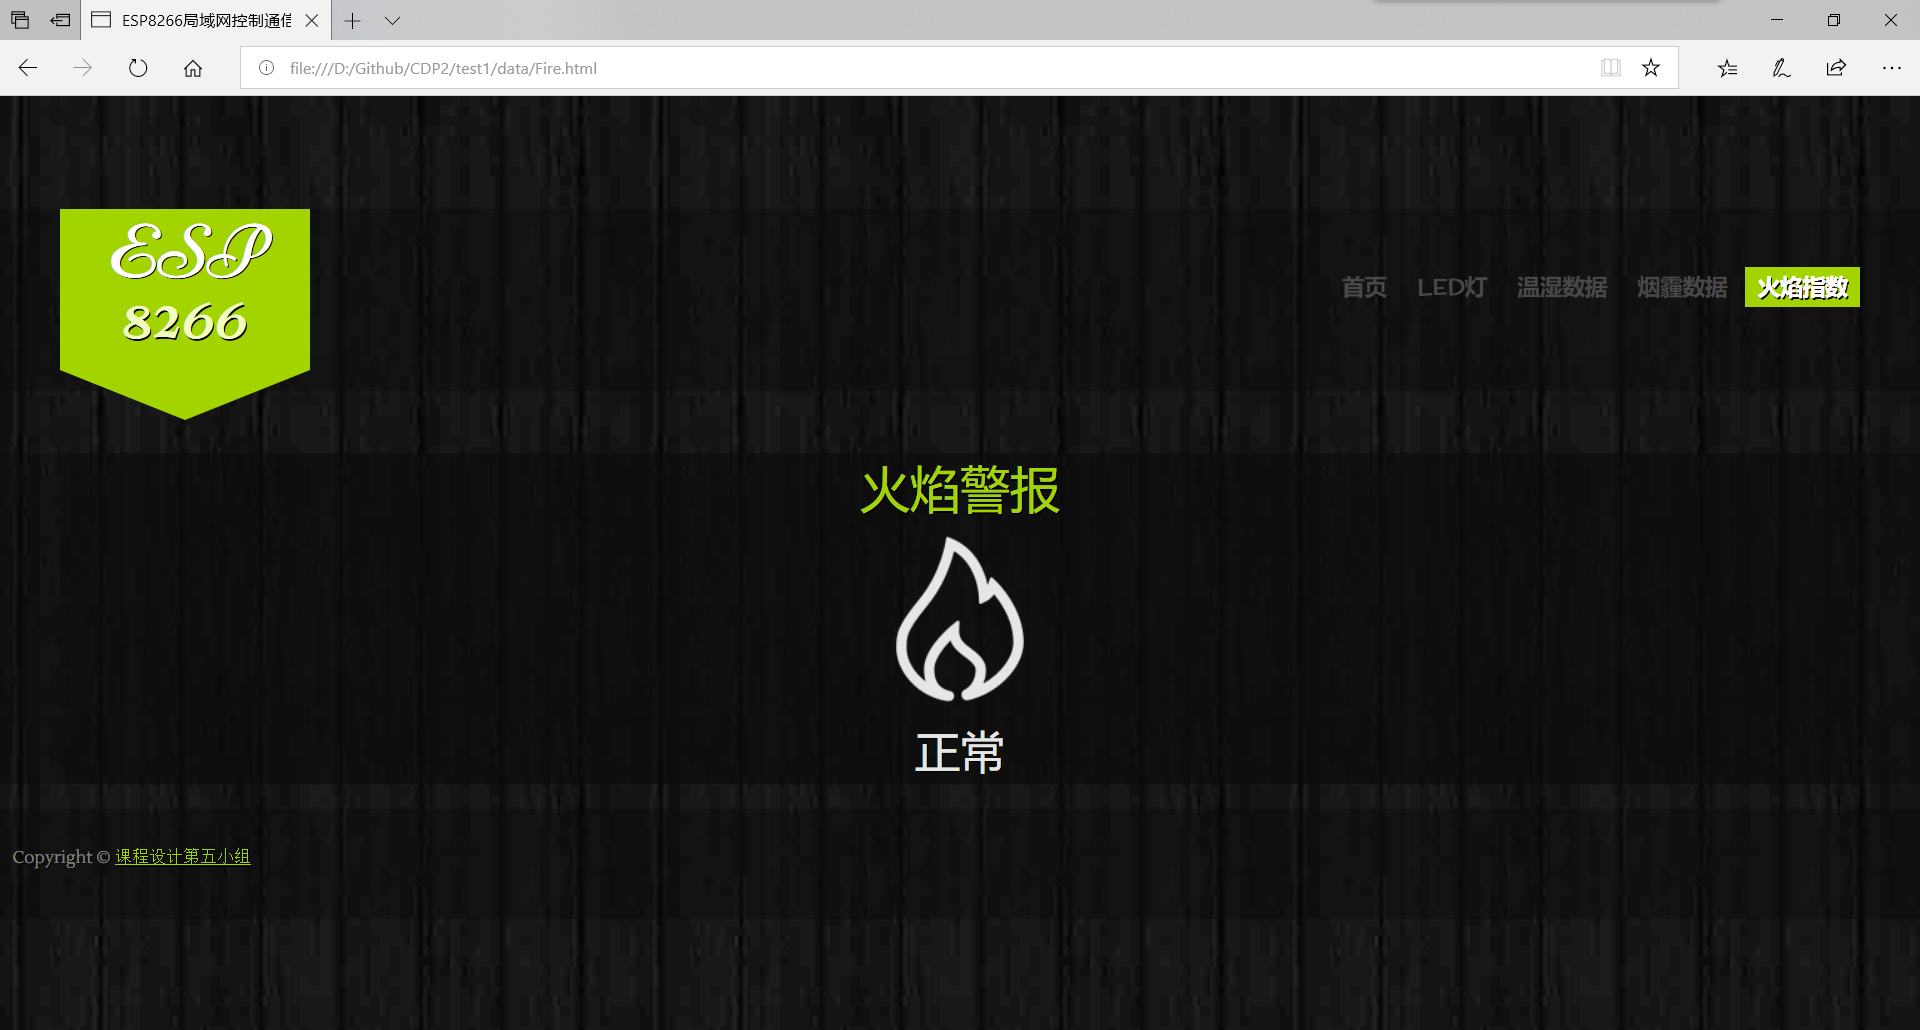
\includegraphics[width=0.95\textwidth]{figures/test/8}   
    \end{minipage}
\end{figure}
	% !Mode:: "TeX:UTF-8"

\chapter{Github成员提交情况}

	% \clearpage

\end{CJK*}                                     % 结束中文字体使用
\end{document}                                 % 结束全文
